%%==================================================
%% chapter01.tex for BIT Master Thesis
%% modified by pinren lu
%% version: 0.1
%% last update: Dec 25th, 2016
%%==================================================
% 相关工作

% 1. 文本生成技术
% 2. 大语言模型生成技术
% 3. 文本分类技术
% 4. 大语言模型文本探测技术
% 5. 本章小结

\chapter{相关工作}
\label{chap:related works}

\section{文本生成技术}
\label{sec:rw-lm}

在当前自然语言处理领域,主流的大语言模型普遍基于 Transformer 框架 \cite{transformer}。自2017年提出以来,该架构因其卓越的并行处理能力和对长距离依赖的建模能力而迅速成为研究的热点。Transformer 通过自注意力机制有效地捕捉输入序列中各部分之间的关系,从而显著提升了在处理大规模文本数据时的训练效率和表达能力。诸如 BERT 和 GPT 系列等知名模型均依托该框架,在多种语言任务中展现出卓越的性能。因此,深入探讨 Transformer 的结构与原理,不仅有助于理解当前大语言模型成功的原因,也为未来研究奠定了重要的理论基础。

Google 公司于2017年提出的一种神经网络模型 Transformer,专为处理序列到序列(Seq2Seq)任务而设计,广泛应用于各种自然语言处理任务。该模型利用自注意力机制来处理输入序列中的关联性,能够有效捕捉长距离依赖关系,而无需依赖循环神经网络或卷积神经网络。此外,Transformer 可以并行处理输入序列中的不同位置,因此在训练和推理过程中,特别是在处理长序列时,展现出更高的效率。Transformer 以独特的编码器-解码器结构为基础,将输入序列转换为输出序列。编码器和解码器均由多个相同的层堆叠而成,每一层都包含多头自注意力机制和前馈神经网络。

\begin{figure}[htb]
	\centering
	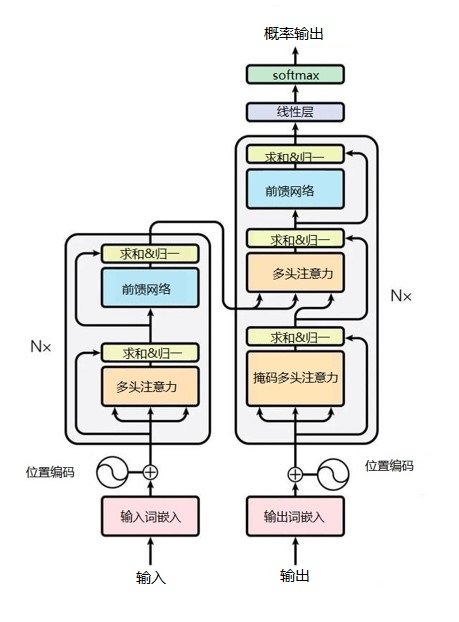
\includegraphics[scale = 0.8]{figures/Transformer2}
	\caption{Transformer 模型结构 \cite{transformer}}
	\label{fig:Transformer2}
\end{figure}

% \subsection{编码器-解码器结构}

(1) 编码器

编码器由 \(N=6\) 个相同的 TransformerEncoderLayer 层构成。每个 TransformerEncoderLayer 层可以再细分为两个子层。在这两个子层中,第一个子层实现了多头自注意力机制,而第二个子层则是一个简单的全连接前馈网络。每个子层后均接有残差连接,随后对经过残差连接的输出进行层归一化。为了确保残差连接的维度相等并便于计算,模型中所有子层及嵌入层的输出向量均设定为 \(d_{\text{model}} = 512\)。

(2) 解码器

解码器同样由 \(N=6\) 个相同的 TransformerDecoderLayer 层组成。每个 TransformerDecoderLayer 层包含三个子层。编码器层中的子层与在解码器其中两个子层的结构大致相似。但是在解码器层中,第三个子层需要获取编码器的输出及解码器层前一个子层的输出,并在该子层内执行多头注意力操作。与编码器层的子层结构相似,解码器层的每个子层后也接有残差连接,随后对经过残差连接的输出向量进行层归一化。Transformer 也将修改放入解码器结构中的自注意力子层中,加入了位置掩码,以防止从前面某个位置获取后面位置的信息。此位置掩码结合位置偏移的设计,确保序列中位置 \(i\) 的元素的预测仅能基于序列中小于 \(i\) 的所有内容。

% \subsection{注意力机制}

% 在 Transformer 中,定义注意力函数为输入为查询和一组键值,然后进行输出的函数,在此之中查询(Query, Q)、键(Key, K)、值(Value, V)和输出都是向量。在注意力函数中,简单地讲,输出实质上是值的加权和。此其中对于每个值的权重由权重相应的键以及查询计算得出。

% (1) 缩放点积注意力

% 在 Transformer 论文中所采用的注意力机制为缩放点积注意力。该机制的输入由查询、键和值组成,其中查询和键的维度均为 \(d_k\),而值的维度为 \(d_v\)。在缩放点积注意力中,我们首先计算查询与所有键向量之间的点积,并随后将这些结果除以 \(\sqrt{d_k}\)。接着,通过 softmax 函数对这些归一化后的向量进行处理,以计算每个值的权重。具体的过程如图 \ref{fig:DotAtt} 所示。

% \begin{figure}[htbp]
% 	\centering
% 	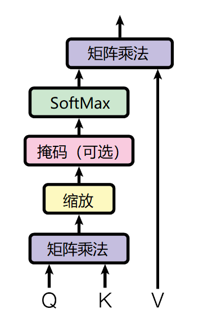
\includegraphics[scale = 0.8]{figures/DotAtt}
% 	\caption{缩放点积注意力 \cite{transformer}}
% 	\label{fig:DotAtt}
% \end{figure}

% 在实际应用中,对于一组待处理的注意力查询,应将这些查询同时进行计算,并将其封装为一个矩阵 \(Q\)。类似地,键和值也被封装为矩阵 \(K\) 和 \(V\)。通过这种方式,计算过程可以通过矩阵乘法进行优化。因此,注意力函数的输出矩阵可以表示为:
% \begin{equation}
% \text{Attention}(Q,K,V) = \text{softmax}(\frac{QK^T}{\sqrt{d_k}})V
% \label{eq3.1}
% \end{equation}

% (2) 多头注意力

% 实际上,如果将键、值和查询统一设定为 \(d_{\text{model}}\) 维度,反而可能导致模型性能下降,相较于将查询、键和值分别投影至 \(d_k\)、\(d_k\) 和 \(d_v\) 维度进行不同的线性变换。在此基础上,注意力函数在每个查询、键和值的投影向量上并行执行,从而生成 \(d_v\) 维的输出值。随后,将这些 \(d_v\) 维的输出值进行连接,并再次进行线性投影,以生成最终输出。具体过程如图 \ref{fig:MultiheadAtt} 所示。

% \begin{figure}[htbp]
% 	\centering
% 	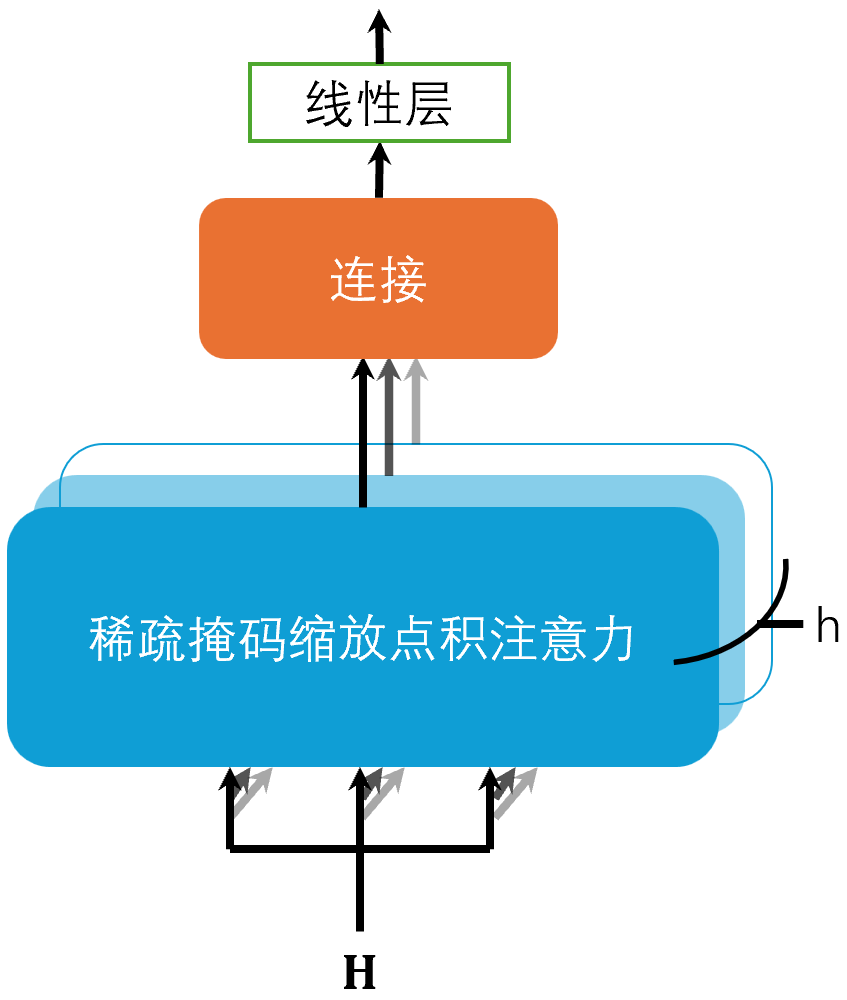
\includegraphics[scale = 0.8]{figures/MultiheadAtt}
% 	\caption{多头注意力 \cite{transformer}}
% 	\label{fig:MultiheadAtt}
% \end{figure}

% 多头注意力的主要优势在于其能够同时关注来自不同位置的信息。相较之下,单一注意力头的使用会导致信息的平均化,从而抑制这一特性。
% \begin{equation}
% \text{MultiHead}(Q, K, V) = \text{Concat}(\text{head}_1, ..., \text{head}_h)W^O
% \label{eq3.2}
% \end{equation}
% \begin{equation}
% \text{head}_i = \text{Attention}(QW_i^Q, KW_i^K, VW_i^V)
% \label{eq3.3}
% \end{equation}
% 在上述公式中,投影操作涉及的参数矩阵包括 \(W_i^Q \in \mathbb{R}^{d_{\text{model}}}\)、\(W_i^K \in \mathbb{R}^{d_{\text{model}} \times d_k}\)、\(W_i^V \in \mathbb{R}^{d_{\text{model}} \times d_v}\) 以及 \(W^O \in \mathbb{R}^{hd_v \times d_{\text{model}}}\)。

% 在 Transformer 架构中,采用了 \(h = 8\) 个并行的注意力层或头。对于每个注意力头,设定其维度为 \(d_k = d_v = d_{\text{model}} / h = 64\)。由于每个头的维度被缩减,因此整体计算成本与具有全维度的单头注意力相当。

% \subsection{位置前馈网络}

% 除了注意力子层外,编码器和解码器的每一层均包含一个全连接的前馈网络,该网络在每个位置上均以相同方式应用。该网络包括两个线性变换,并在其间引入一个线性整流单元(ReLU)激活函数。具体表达式为:
% \begin{equation}
% \text{FFN}(x) = \max(0, xW_1 + b_1)W_2 + b_2
% \label{eq3.4}
% \end{equation}

% 尽管在不同位置上应用的线性变换相同,但在层与层之间所使用的参数却是各异的。可以将其视作两个内核大小为 \(1\) 的卷积操作。输入和输出的维度均为 \(d_{\text{model}} = 512\),而内部层的维度为 \(d_{ff} = 2048\)。

% \subsection{嵌入层与 Softmax 函数}

% 与其他序列转换模型相似,Transformer 采用学习嵌入技术,将输入序列和输出序列中的词汇映射为维度为 \(d_{\text{model}}\) 的向量。此外,模型还利用常规的学习线性变换及 Softmax 函数,将解码器的输出转化为对下一个词汇的预测概率。在我们的模型中,两个嵌入层与预 Softmax 线性变换之间共享相同的权重矩阵。在嵌入层中,这些权重会乘以因子 \(\sqrt{d_{\text{model}}}\)。此外,也存在将 log-softmax 函数替代 Softmax 函数的做法。

% \subsection{位置编码}

% 由于 Transformer 模型不采用递归或卷积结构,为了使模型能够有效利用序列的顺序信息,必须引入某种形式的标记在序列中相对或绝对位置的信息。因此,我们在编码器和解码器堆栈的输入嵌入中添加了“位置编码”。位置编码的维度与嵌入相同,即 \(d_{\text{model}}\),从而可以将两者直接相加。位置编码的形式多种多样,既可以通过模型学习得到,也可以通过预定义的公式计算得出。

% 在 Transformer 中,采用了不同频率的正弦和余弦函数来生成位置编码,具体表达式为:
% \begin{equation}
% \begin{aligned}
% \text{PE}(pos,2i) &= \sin \left ( \frac{pos}{10000^{2i/d_{\text{model}}}} \right ) \\
% \text{PE}(pos,2i+1) &= \cos \left ( \frac{pos}{10000^{2i/d_{\text{model}}}} \right )
% \end{aligned}
% \label{eq3.5}
% \end{equation}
% 其中 \(pos\) 表示位置,\(i\) 表示维度。换言之,位置编码的每个维度对应于一条正弦曲线,其波长形成从 \(2\pi\) 到 \(10000 \cdot 2\pi\) 的几何级数。选择这种函数的原因在于我们假设它能够使模型更容易地学习通过相对位置进行计算,因为对于任何固定的偏移量 \(k\),\(\text{PE}_{pos+k}\) 可以表示为 \(\text{PE}_{pos}\) 的线性函数。

% \subsection{线性层}

% 在数据经过 log-softmax 函数处理后,将通过一层线性层将维度为 \(d_{\text{model}}\) 的向量转换为一个维度等于词汇表大小的向量,该向量用于表示对下一个预测词汇的概率分布。

\section{预训练语言模型技术}

近年来,自然语言处理(Natural Language Processing, NLP)领域经历了显著的进展,其中预训练语言模型(Pre-trained Language Models, PLMs)的研究为该领域的发展提供了重要支持。预训练语言模型的核心思想是首先在进行预训练阶段的训练,基于大规模数据集的训练以获得模型参数,此举可使模型获得对于数据初步的认知,随后利用这些经过训练的模型来在具体的下游任务数据上进行微调。预训练语言模型的早期研究甚至可以追溯到 NNLM \cite{NNLM} 和 word2Vec \cite{mikolov2013efficientestimationwordrepresentations}。2017 年,Vaswani 等人 \cite{transformer} 提出了 Transformer 架构,这一架构的引入显著提升了多种 NLP 任务的性能,使 Transformer 成为众多预训练语言模型的基础。在基于 Transformer 的编码器架构中,Radford 等人 \cite{gpt} 提出了 GPT 模型,该模型真正实现了预训练-微调的框架,避免了将词嵌入从模型中提取的过程。目前,GPT 模型的应用取得了显著成功,各种大型 GPT 模型层出不穷,为 NLP 等领域注入了新的活力。同时,Devlin 等人 \cite{devlin_bert_2019} 基于 Transformer 的编码器提出了 BERT 模型,成为目前自然语言处理领域中应用最广泛的模型之一。BERT 在预训练阶段,采用了掩码语言模型(Masked Language Model, MLM)的方法。这种方法是从输入文本中通过随机掩盖某些词元,此后利用除了被掩盖词元外的上下文信息进行预测,从而实现对模型的训练。继 GPT 和 BERT 之后,研究人员还提出了 XLNet \cite{XLNet}、RoBERTa \cite{liu_roberta_2019}、DeBERTa \cite{he_deberta_2021}、ERNIE \cite{sun2019ernieenhancedrepresentationknowledge}、T5 \cite{T5} 和 BART \cite{lewis-etal-2020-bart} 等多种预训练语言模型。本节将介绍本文所采用的 RoBERTa 和 DeBERTa 模型的基础预训练语言模型 BERT 模型。

% 写写 BERT 吧
BERT(Bidirectional Encoder Representations from Transformers)\cite{devlin_bert_2019} 是由 Google 提出的预训练模型。该模型在机器阅读理解的顶级基准测试 SQuAD1.1 \cite{rajpurkar2016squad100000questionsmachine} 中展现了卓越的性能:在所有两个评估指标上均显著超越了人类表现,并在 11 项不同的 NLP 测试中创造了最新的状态-of-the-art(SOTA)成绩。其中,GLUE 基准 \cite{wang2019gluemultitaskbenchmarkanalysis} 的得分提升至 80.4\%(绝对改进 7.6\%),而 MultiNLI 数据集 \cite{williams2018broadcoveragechallengecorpussentencemultinli} 的准确率达到 86.7\%(绝对改进 5.6\%),标志着这一模型在自然语言处理领域的里程碑式成就。BERT 在 Transformer 架构的基础上引入了预训练与微调的策略,使得模型能够在预训练阶段学习通用的语言表示,并在特定任务中进行微调,从而显著提高了模型的适应性与性能。因此,尽管 BERT 并非首个预训练模型,但在预训练模型的发展历程中,其重要性不容忽视,具有里程碑式的意义。

\subsection{BERT 结构}

BERT 在 Transformer 的基础上并未进行大量改进,而是采用了 Transformer 编码器的结构作为其核心架构。其总体结构如图 \ref{fig:BERT} 所示,多个 Transformer 编码器层逐层堆叠构成了 BERT 的整体框架。在原始论文中,作者分别构建了两种 BERT 模型,采用了 12 层和 24 层的 Transformer 编码器,分别对应于 110M 和 340M 的总参数量。

\begin{figure}[htb]
	\centering
	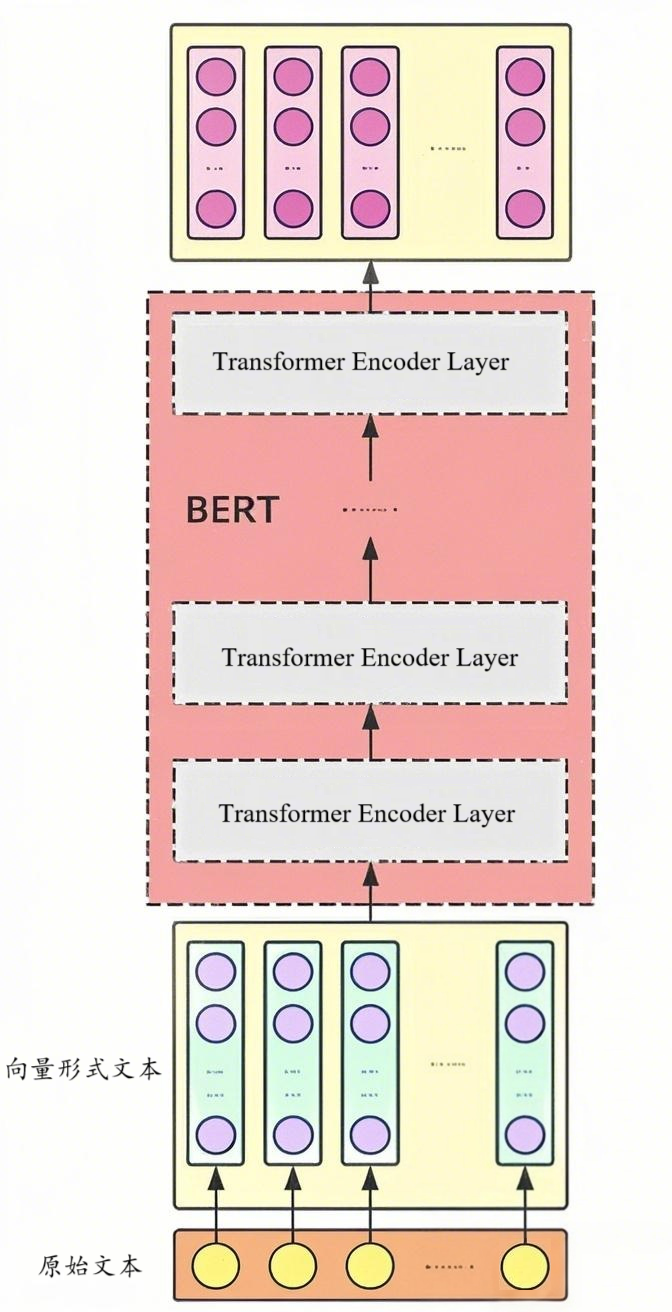
\includegraphics[scale = 0.5]{figures/bert.png}
	\caption{BERT 架构图 \cite{devlin_bert_2019}}
	\label{fig:BERT}
\end{figure}

\subsubsection{嵌入}

对于 BERT 而言,其在嵌入(Embedding)方面的显著改进是一个关键创新。为了使 BERT 能够有效处理多种下游任务,其输入表示能够清晰地区分单个句子和句子对(例如,〈问题, 答案〉)在同一词元序列中。

在 BERT 中,每个序列的首个词元始终是一个特殊的非正文的分类词元([CLS]),该标记的最终向量可视为整句话的语义表示,进而用于下游的分类任务等。由于该标记本身并非正文内容,因此缺乏明显的语义信息,使用它的最终向量能恰好地在文本中整合各个词的语义。在经过 BERT 这一预训练语言模型的处理后,所有词的信息同时也被融合进入了每个词的嵌入中,从而更准确地反映其语义。在 BERT 的执行过程中,句子对会被合并成一个序列然后由 BERT 模型处理。区分句子大致分为两步。首先,在原始输入文本中加入特殊标记([SEP])分开两个句子。其次,BERT 将句子嵌入融合到每个词元生成的向量中,以表明其为哪个句子。

\begin{figure}[htb]
	\centering
	\includegraphics[width=0.9\linewidth]{figures/bert_Input_Embeddings.jpg}
	\caption{BERT 嵌入(Embedding)示意图 \cite{devlin_bert_2019}}
	\label{fig:BERT-embedding}
\end{figure}

对于每个给定的词元,其输入表示(input representation)是通过对相应的词元(token)、段落(segment)和位置(position)嵌入进行加和来构建的。该结构的可视化展示见图 \ref{fig:BERT-embedding}。

\subsubsection{预训练与微调}

BERT 研究的主要贡献在于其二阶段训练过程的有效推广,该过程分为预训练(pretraining)和微调(finetuning)两个阶段,训练流程的示意图如图 \ref{fig:BERT-OverAll} 所示。在预训练阶段,BERT 通过大规模的无标注文本数据学习语言的深层次表示,采用了带掩码的语言模型(Masked Language Model, MLM)和下一句预测(Next Sentence Prediction, NSP)两种任务,从而使模型能够理解上下文的双向信息。在微调阶段,BERT 通过在少量标注数据上进行训练,能够针对特定任务进行调整,进而高效适应多种自然语言处理任务,如文本分类、问答系统和命名实体识别等。

\begin{figure}[htb]
	\centering
	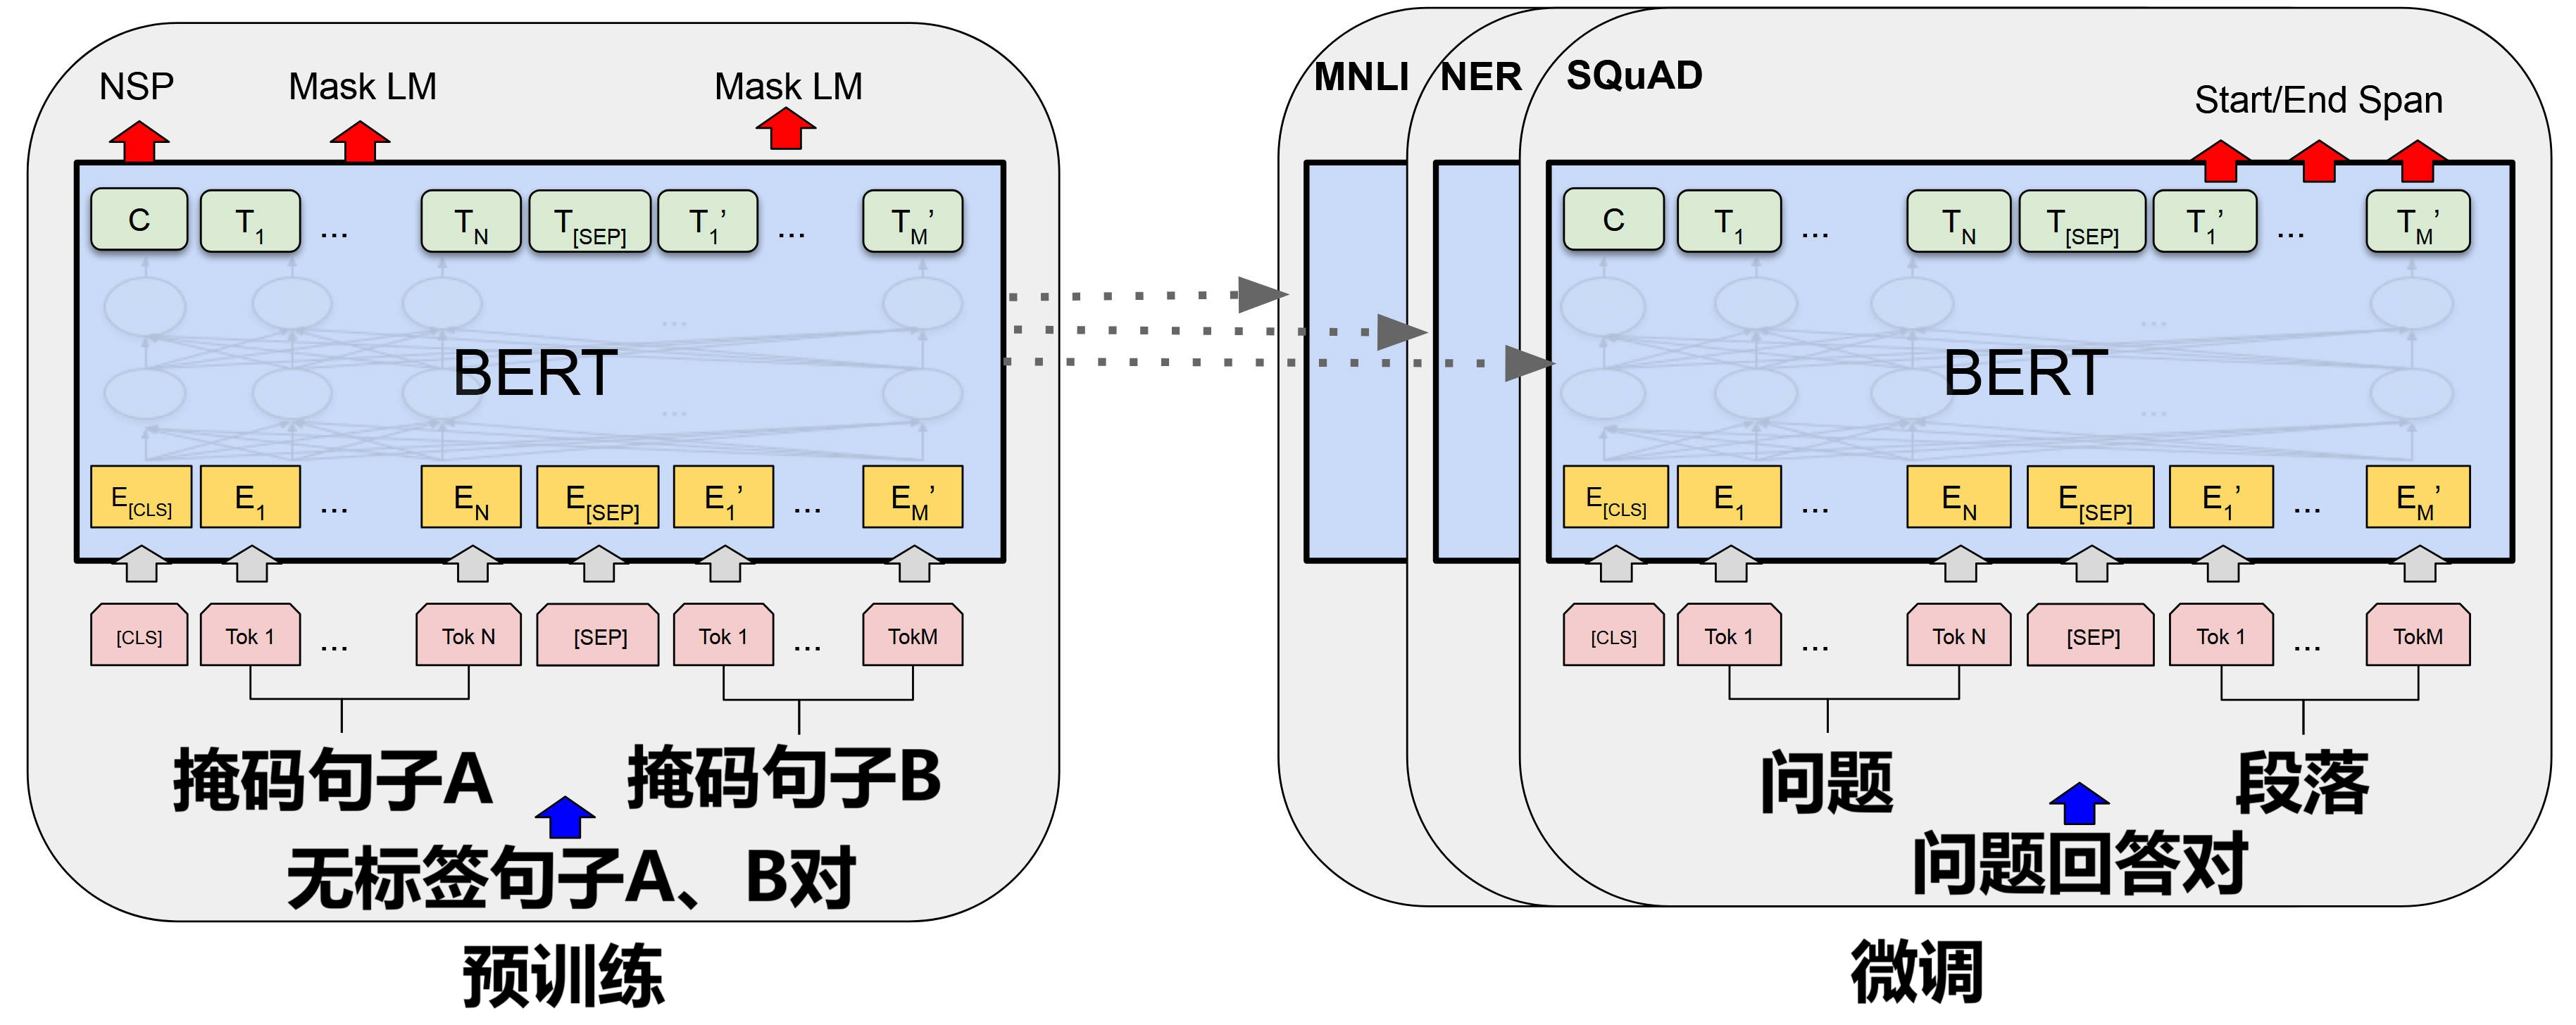
\includegraphics[width=0.9\linewidth]{figures/BERT_Overall.jpg}
	\caption{BERT 训练过程示意图 \cite{devlin_bert_2019}}
	\label{fig:BERT-OverAll}
\end{figure}

这种预训练-微调的二阶段训练范式显著提高了模型在多种自然语言处理(NLP)任务上的性能,标志着该领域的一次重要变革。BERT 的成功激励了大量基于 Transformer 架构的预训练模型的后续研发,例如本文将使用的 RoBERTa 和 DeBERTa,以及其他在 BERT 模型基础上进行改进的模型。这些模型在不同任务中展现出更高的效率和准确性。通过这些创新,BERT 不仅推动了学术界对预训练模型的深入研究,也促进了工业界在实际应用中的广泛采用。

\subsection{RoBERTa 模型}
\label{sec:method-pretrain-roberta}

RoBERTa \cite{liu_roberta_2019}(Robustly Optimized BERT Approach)在 BERT \cite{devlin_bert_2019} 模型的基础上进行了多方面的优化,显著提升了模型的整体性能。

在训练策略方面,原始 BERT 模型存在训练不足的问题。为了解决这一缺陷,RoBERTa 通过延长训练步数、采用更大的批次进行训练,并在更广泛的数据集上进行训练。在实验中,较大的批次训练 BERT 模型的结果表明,这种策略能够有效降低训练的困惑度(perplexity),并提高下游任务的准确率。此外,大批次训练更易于通过分布式数据并行实现,从而显著提升了训练效率。

在训练数据的选择上,RoBERTa 使用了总计 160GB 的未压缩文本,涵盖多种语料库,这一数据量远超 BERT 原始训练所用的 16GB。此结果充分表明数据量和多样性在预训练过程中的重要性。此外,BERT 原始实现中,掩码是在数据预处理阶段一次性生成的,形成了静态掩码。尽管通过数据复制增加掩码的多样性,但该方法仍存在局限性。相较之下,RoBERTa 采用了动态掩码机制,即在每次向模型输入序列时生成新的掩码模式。这一方法在长时间训练或处理大规模数据集时表现出明显优势,不仅提高了训练效率,还在实验中显示出相较于静态掩码更优或相当的性能。

在模型输入格式的优化方面,原始 BERT 模型在训练时使用了下一个句子预测(NSP)任务,以提升下游任务的性能。然而,相关研究 \cite{Lample2019CrosslingualLM, Yang2019XLNetGA, Joshi2019SpanBERTIP} 对这一任务提出了质疑。RoBERTa 经过对比实验发现,去除 NSP 损失并采用从单个文档中采样完整句子作为输入,能够匹配或略微提升下游任务的性能。具体而言,限制序列来自单个文档的 DOC-SENTENCES 格式表现优于从多个文档打包的 FULL-SENTENCES 格式,但为了便于与相关研究的比较,最终 RoBERTa 选择了从多个文档打包的 FULL-SENTENCES 格式。此外,RoBERTa 不再使用 BERT 原有的两文档片段拼接并添加 NSP 损失的输入格式,而是采用从一个或多个文档中连续采样完整句子的方式,确保输入总长度不超过 512 个标记。这一格式有助于模型学习长距离依赖关系,从而增强文本理解能力。

在文本编码的改进方面,BERT 原实现使用了一个大小为 30K 的字符级字节对编码 \cite{BPE}(BPE)词汇表,并需要进行启发式分词规则的预处理。RoBERTa 借鉴其他研究,采用了一个包含 50K 子词单元的更大字节级 BPE 词汇表,这一方法无需额外的预处理或分词。尽管在某些任务上性能略有下降,但由于其通用编码方案的优势,RoBERTa 仍被广泛应用于后续的实验中。

通过以上对 BERT 的改进,RoBERTa 在多个自然语言处理任务中展现出卓越的性能,为后续研究提供了强有力的支持。

在本文中,采用 RoBERTa-base 和 RoBERTa-Large 两种大小的 RoBERTa 模型,其参数如表 \ref{tab:roberta-parameter} 所示。表中的参数包括 Transformer 层数、隐藏层维度、注意力头数以及总参数量。这些参数的设计反映了模型的复杂性及其学习能力。较大的模型(RoBERTa-Large)在处理更复杂的语言任务时,能够更好地捕捉深层次的语义关系和上下文信息,而较小的模型(RoBERTa-Base)则在计算效率和资源消耗上具有一定的优势。通过对比这两种模型的性能,我们能够深入探讨不同规模模型在文本理解和生成任务中的表现差异,从而为后续研究提供有价值的参考。

\begin{table*}[htbp]
\centering
\caption{ RoBERTa-Base 和 RoBERTa-Large 参数} \label{tab:roberta-parameter}
\begin{tabular}{lcc}
\toprule
               & \multicolumn{1}{l}{\textbf{RoBERTa-Base} \cite{liu_roberta_2019}} & \multicolumn{1}{l}{\textbf{RoBERTa-Large} \cite{liu_roberta_2019}} \\ \midrule
Transformer 层数 & 12                                        & 24                                         \\
隐藏层维度          & 768                                       & 1024                                       \\
注意力头数          & 12                                        & 16                                         \\
总参数量           & 125M                                      & 355M                                      \\ \bottomrule
\end{tabular}
\end{table*}

\subsection{DeBERTa 模型}
\label{sec:method-pretrain-deberta}

目前 DeBERTa 系列模型公开的论文仅有 DeBERTa 模型 \cite{he_deberta_2021} 和 DeBERTa V3 模型 \cite{he2023debertav3improvingdebertausing},我们的实验中将会使用 DeBERTa V3 模型,本节将会对 DeBERTa 模型对于 BERT \cite{devlin_bert_2019} 和 RoBERTa 模型 \cite{liu_roberta_2019} 的改进进行介绍。

\subsubsection{DeBERTa 模型}

DeBERTa 模型 \cite{he_deberta_2021} 是预训练语言模型演进过程中的一项重要成果,相较于本文先前提及的 RoBERTa 和 BERT,其在多个方面进行了显著改进。这些改进主要体现在注意力机制、掩码解码器以及训练方法等方面,从而显著提升了模型的性能和泛化能力。

在注意力机制的设计上,BERT 和 RoBERTa 将每个单词表示为其词嵌入(内容)与位置嵌入的和,这种表示方式在一定程度上融合了内容和位置信息。相较之下,DeBERTa 采用了一种创新的解耦注意力机制,将每个单词分别编码为两个独立的向量,分别代表内容和位置。在计算单词间的注意力权重时,DeBERTa 利用基于内容和相对位置的解耦矩阵进行独立计算。这种方法使得模型能够更精细地捕捉单词之间的关系。以句子 “The dog chased the cat” 为例,当分析 “dog” 与 “cat” 之间的关系时,DeBERTa 不仅考虑它们的语义内容,还能基于相对位置更准确地判断其依赖关系。相较而言,BERT 和 RoBERTa 在处理这种复杂关系时则显得不够细致。

对于序列中位置为 \(i\) 的词元(token),DeBERTa 采用两个向量进行表示,分别为 \(\mathbf{H}_{i}\) 和 \(\mathbf{P}_{i|j}\)。其中,\(\mathbf{H}_{i}\) 表示该词元的内容信息,而 \(\mathbf{P}_{i|j}\) 则表示该词元与位置为 \(j\) 的词元之间的相对位置关系。词元 \(i\) 与 \(j\) 之间的交叉注意力分数的计算可以被分解为四个组成部分,具体如下:
\begin{align}
\label{eq:deberta-attention}
\begin{split}
\mathbf{A}_{i, j} & = \{\mathbf{H}_{i}, \mathbf{P}_{i | j}\} \times \{\mathbf{H}_{j}, \mathbf{P}_{j | i}\}^{\intercal} \\
& = \mathbf{H}_{i}\mathbf{H}_{j}^{\intercal}+\mathbf{H}_{i}\mathbf{P}_{j | i}^{\intercal}+\mathbf{P}_{i | j}\mathbf{H}_{j}^{\intercal}+\mathbf{P}_{i | j}\mathbf{P}_{j | i}^{\intercal}.
\end{split}
\end{align}

换言之,单词对之间的注意力权重可以通过将基于其内容和位置的解耦矩阵应用于四个注意力分数的求和来计算。这四个分数分别对应于内容对内容、内容对位置、位置对内容以及位置对位置的注意力。

在 DeBERTa 之前,相对位置编码的方法在计算注意力权重时,通常依赖于独立的嵌入矩阵来确定相对位置偏差 \cite{Shaw2018SelfAttentionWR, Huang2018MusicTG}。这相当于仅利用公式 \ref{eq:deberta-attention} 中的内容对内容和内容对位置这两项计算注意力权重。因为单词对的注意力权重不仅依赖于其内容信息,还受到相对位置的影响,因此位置对内容的项同样十分重要。由于在 DeBERTa 中处理位置的方式是相对位置嵌入,因此位置对位置的该项在 DeBERTa 的中被认为提供的额外信息有限,因此从公式 \ref{eq:deberta-attention} 中去除了该项。

以单头注意力为例,标准的自注意力操作 \cite{transformer} 可以表示为:
\begin{align}
\mathbf{Q} = \mathbf{HW_{q}}, \mathbf{K} &= \mathbf{HW_{k}}, V = \mathbf{HW_{v}}, \mathbf{A} = \frac{\mathbf{QK}^{\intercal}}{\sqrt{d}} \\
\mathbf{H_{o}} &= \text{softmax}(\mathbf{A})\mathbf{V}
\label{eq:transformer-attention1}
\end{align}
其中,$\mathbf{H} \in \mathbb{R}^{N×d}$ 表示输入的隐藏向量,$\mathbf{H_{o}} \in \mathbb{R}^{N×d}$ 是自注意力的输出,$\mathbf{W_{q}}$、$\mathbf{W_{k}}$、$\mathbf{W_{v}} \in \mathbb{R}^{d×d}$ 是投影矩阵,$\mathbf{A} \in \mathbb{R}^{N×N}$ 是注意力矩阵,$N$ 是输入序列的长度,$d$ 是隐藏状态的维度。

记 $k$ 为最大相对距离,$\delta(i, j) \in [0, 2k)$ 为从词元 $i$ 到词元 $j$ 的相对距离,其定义为:
\begin{align}
\delta(i, j)=\begin{cases}
0, & \text{当~} i - j \leq -k \\
2k - 1, & \text{当~} i - j \geq k \\
i - j + k, & \text{其他情况}
\end{cases}
\label{eq:deberta-distance}
\end{align}

在 DeBERTa 中,带有相对位置偏差的解耦自注意力机制可以用公式 \ref{eq:deberta-dis-att} 来表示。在该公式中,\(\mathbf{Q}_{c}\)、\(\mathbf{K}_{c}\) 和 \(\mathbf{V}_{c}\) 分别是通过投影矩阵 \(\mathbf{W}_{q,c}\)、\(\mathbf{W}_{k,c}\) 和 \(\mathbf{W}_{v,c} \in \mathbb{R}^{d \times d}\) 生成的投影内容向量。此外,\(\mathbf{P} \in \mathbb{R}^{2k \times d}\) 表示在所有层中共享的相对位置嵌入向量,该向量在正向传播过程中保持不变。相对位置向量 \(\mathbf{Q}_{r}\) 和 \(\mathbf{K}_{r}\) 则是通过投影矩阵 \(\mathbf{W}_{q,r}\) 和 \(\mathbf{W}_{k,r} \in \mathbb{R}^{d \times d}\) 生成的。
\begin{align} \label{eq:deberta-dis-att}
\begin{split}
    \mathbf{Q}_c = \mathbf{H} \mathbf{W}_{q,c}, 
    \mathbf{K}_c &= \mathbf{H} \mathbf{W}_{k,c}, 
    \mathbf{V}_c = \mathbf{H} \mathbf{W}_{v,c}, 
    \mathbf{Q}_r = \mathbf{P} \mathbf{W}_{q,r}, 
    \mathbf{K}_r = \mathbf{P} \mathbf{W}_{k,r} \\
    \tilde{\mathbf{A}}_{i,j} &= \underbrace{\mathbf{Q}^{c}_{i}{\mathbf{K}^{c}_{j}}^{\intercal}}_{\text{(a) content-to-content}}  
    + \underbrace{\mathbf{Q}^{c}_{i}{{\mathbf{K}^{r}_{\delta(i,j)}}^{\intercal}}}_{\text{(b) content-to-position}}
    + \underbrace{\mathbf{K}^{c}_{j}{{\mathbf{Q}^{r}_{\delta(j,i)}}^{\intercal}}}_{\text{(c) position-to-content}} \\
    \mathbf{H_o} &= \text{softmax}(\frac{\tilde{\mathbf{A}}}{\sqrt{3d}})\mathbf{V}_c
\end{split}
\end{align}
在此,\(\tilde{\mathbf{A}}_{i,j}\) 表示注意力矩阵 \(\tilde{\mathbf{A}}\) 的一个元素,具体对应于词元 \(i\) 到词元 \(j\) 的注意力分数。具体而言,\(\mathbf{Q}_{i}^{c}\) 是矩阵 \(\mathbf{Q}_{c}\) 的第 \(i\) 行,而 \(\mathbf{K}_{j}^{c}\) 则是矩阵 \(\mathbf{K}_{c}\) 的第 \(j\) 行。同时,\(\mathbf{K}_{\delta(i,j)}^{r}\) 表示相对位置向量 \(\mathbf{K}_{r}\) 中与相对距离 \(\delta(i,j)\) 对应的第 \(\delta(i,j)\) 行,\(\mathbf{Q}_{\delta(j,i)}^{r}\) 则是与相对距离 \(\delta(j,i)\) 对应的第 \(\delta(j,i)\) 行。值得注意的是,DeBERTa 在此使用 \(\delta(j,i)\) 而非 \(\delta(i,j)\),原因在于对于特定位置 \(i\),位置对内容的计算实际上是基于位置 \(j\) 的键内容相对于位置 \(i\) 的查询位置的注意力权重。因此,此时相对距离应为 \(\delta(j,i)\)。位置对内容项的计算公式为 \(\mathbf{K}_{j}^{c} \cdot {\mathbf{Q}_{\delta(j,i)}^{r}}^{\intercal}\),而内容对位置的计算方式则类似。

最后,对注意力矩阵 \(\tilde{\mathbf{A}}\) 应用一个缩放因子 \(\frac{1}{\sqrt{3d}}\)。这一缩放因子在模型训练的稳定性方面发挥了关键作用 \cite{transformer},尤其是在处理大规模预训练语言模型时,其重要性愈加突出。

\begin{algorithm}[htb]
\caption{解耦注意力(Disentangled Attention)}
\label{algo:DA}
%\SetAlgoLined
 \begin{algorithmic}[1]
    \Require {隐藏状态 $\mathbf{H}$, 相对距离嵌入 $\mathbf{P}$, 相对距离矩阵 $\mathbf{\delta}$.}
    内容投影矩阵 $\mathbf{W}_{k,c}$, $\mathbf{W}_{q,c}$, $\mathbf{W}_{v,c}$,
    位置投影矩阵 $\mathbf{W}_{k,r}$, $\mathbf{W}_{q,r}$.
    \Ensure $\mathbf{H}_o$

    \State {$\mathbf{K}_c = \mathbf{H}\mathbf{W}_{k,c}$, $\mathbf{Q}_c = \mathbf{H}\mathbf{W}_{q,c}$, $\mathbf{V}_c = \mathbf{H}\mathbf{W}_{v,c}$,   $\mathbf{K}_r = \mathbf{P}\mathbf{W}_{k,r}$, $\mathbf{Q}_r = \mathbf{P}\mathbf{W}_{q,r}$}
    \State {$\mathbf{A}_{c\rightarrow c} = \mathbf{Q}_c \mathbf{K}_c^{\intercal}$} 
    \For{$i=0,...,N-1$} 
        \State {$\tilde{\mathbf{A}}_{c\rightarrow p}[i,:] = \mathbf{Q}_{c}[i,:] \mathbf{K}_r^{\intercal}$} 
    \EndFor
    \For {$i=0,...,N-1$}
        \For {$j=0,...,N-1$}
        \State {$\mathbf{A}_{c\rightarrow p}[i,j] = \tilde{\mathbf{A}}_{c\rightarrow p}[i,\mathbf{\delta}[i,j]]$} 
        \EndFor
    \EndFor
    \For{$j=0,...,N-1$}
        \State {$\tilde{\mathbf{A}}_{p\rightarrow c}[:,j] = \mathbf{K}_{c}[j,:] \mathbf{Q}_r^{\intercal}$} 
    \EndFor
    \For {$j=0,...,N-1$}
        \For {$i=0,...,N-1$}
        \State {$\mathbf{A}_{p\rightarrow c}[i,j] = \tilde{\mathbf{A}}_{p\rightarrow c}[\mathbf{\delta}[j,i],j]$} 
        \EndFor
    \EndFor
    \State {$\tilde{\mathbf{A}}=\mathbf{A}_{c\rightarrow c} + \mathbf{A}_{c\rightarrow p} + \mathbf{A}_{p\rightarrow c}$}
    \State {$\mathbf{H}_o = \text{softmax}(\frac{\tilde{\mathbf{A}}}{\sqrt{3d}})\mathbf{V}_c$}
 \end{algorithmic}

\end{algorithm}

DeBERTa 采用了一种高效的实现方法。在其之前的研究中,对于长度为 \(N\) 的输入序列,每个词元的相对位置嵌入需要 \(O(N^{2}d)\) 的空间复杂度 \cite{Shaw2018SelfAttentionWR, Huang2018MusicTG, Dai2019TransformerXLAL}。然而,以内容对位置的计算为例,DeBERTa 观察到相对距离 \(\delta(i, j)\) 的范围为 \([0, 2k)\),并且所有可能的相对位置嵌入实际上构成了矩阵 \(\mathbf{K}_{r} \in \mathbb{R}^{2k \times d}\) 的一个子集。因此,我们能够在所有查询的注意力计算过程中重用 \(\mathbf{K}_{r}\),从而显著降低了存储需求。

在 DeBERTa 中,预训练阶段将最大相对距离 \(k\) 设置为 512。解耦的注意力权重可以通过算法 \ref{algo:DA} 高效计算。设 \(\delta\) 为根据公式 \ref{eq:deberta-distance} 得到的相对位置矩阵,其中 \(\delta[i, j] = \delta(i, j)\)。在此过程中,我们并不为每个查询分配独立的相对位置嵌入矩阵,而是通过将每个查询向量 \(\mathbf{Q}_{c}[i, :]\) 乘以 \(\mathbf{K}_{r}^{\intercal} \in \mathbb{R}^{d \times 2k}\)(如算法 \ref{algo:DA} 的第 3-5 行),并利用相对位置矩阵 \(\delta\) 作为索引来提取注意力权重(如算法 \ref{algo:DA} 的第 6-10 行)。为了计算位置对内容的注意力分数,我们通过将每个键向量 \(\mathbf{K}_{c}[j, :]\) 乘以 \(\mathbf{Q}_{r}^{T}\) 来获得注意力矩阵 \(\tilde{\mathbf{A}}_{p \to c}[:, j]\) 的列向量(如算法 \ref{eq:deberta-distance} 的第 11-13 行),并最终通过相对位置矩阵 \(\delta\) 作为索引提取相应的注意力分数(如算法 \ref{algo:DA} 的第 14-18 行)。通过这种方法,我们避免了为每个查询分配内存以存储相对位置嵌入,从而将空间复杂度降低至 \(O(kd)\),仅需存储 \(\mathbf{K}_{r}\) 和 \(\mathbf{Q}_{r}\)。

此外,DeBERTa 还采用了掩码语言建模(Masked Language Modeling, MLM)作为预训练策略。在这一过程中,模型通过利用周围未被掩码的词汇来预测被掩码的词。DeBERTa 在掩码语言模型任务中充分考虑了位置信息及其上下文词的内容。在解耦注意力机制,上下文词的内容和相对位置被提到了相当重要的位置,但这些词的绝对位置却并没有被该方法充分使用。多数情况下,精确预测高度依赖于绝对位置信息。

\begin{figure*}[htbp]
\centering  
\subfloat[BERT 解码层]{
    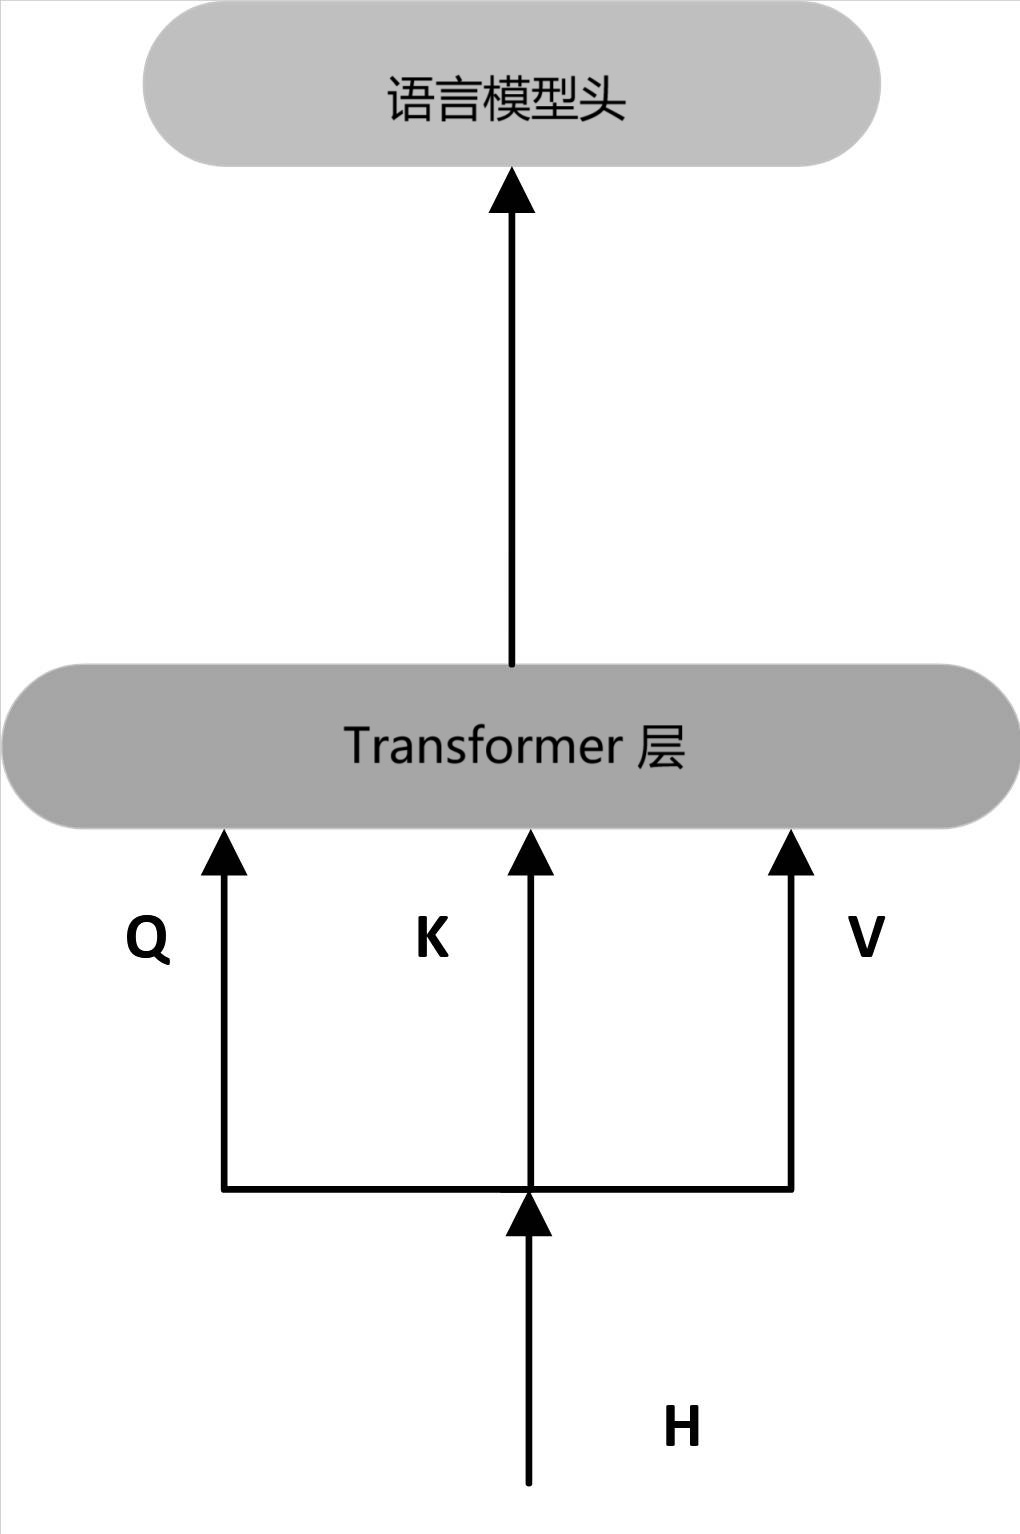
\includegraphics[trim={0.5mm 0.5mm 0.5mm 0.5mm},clip,width=0.35\linewidth]{figures/Model_BERT_S.jpg}
    % \label{fig:bert-a}
}
\hfill
\subfloat[改进的遮掩解码]{
    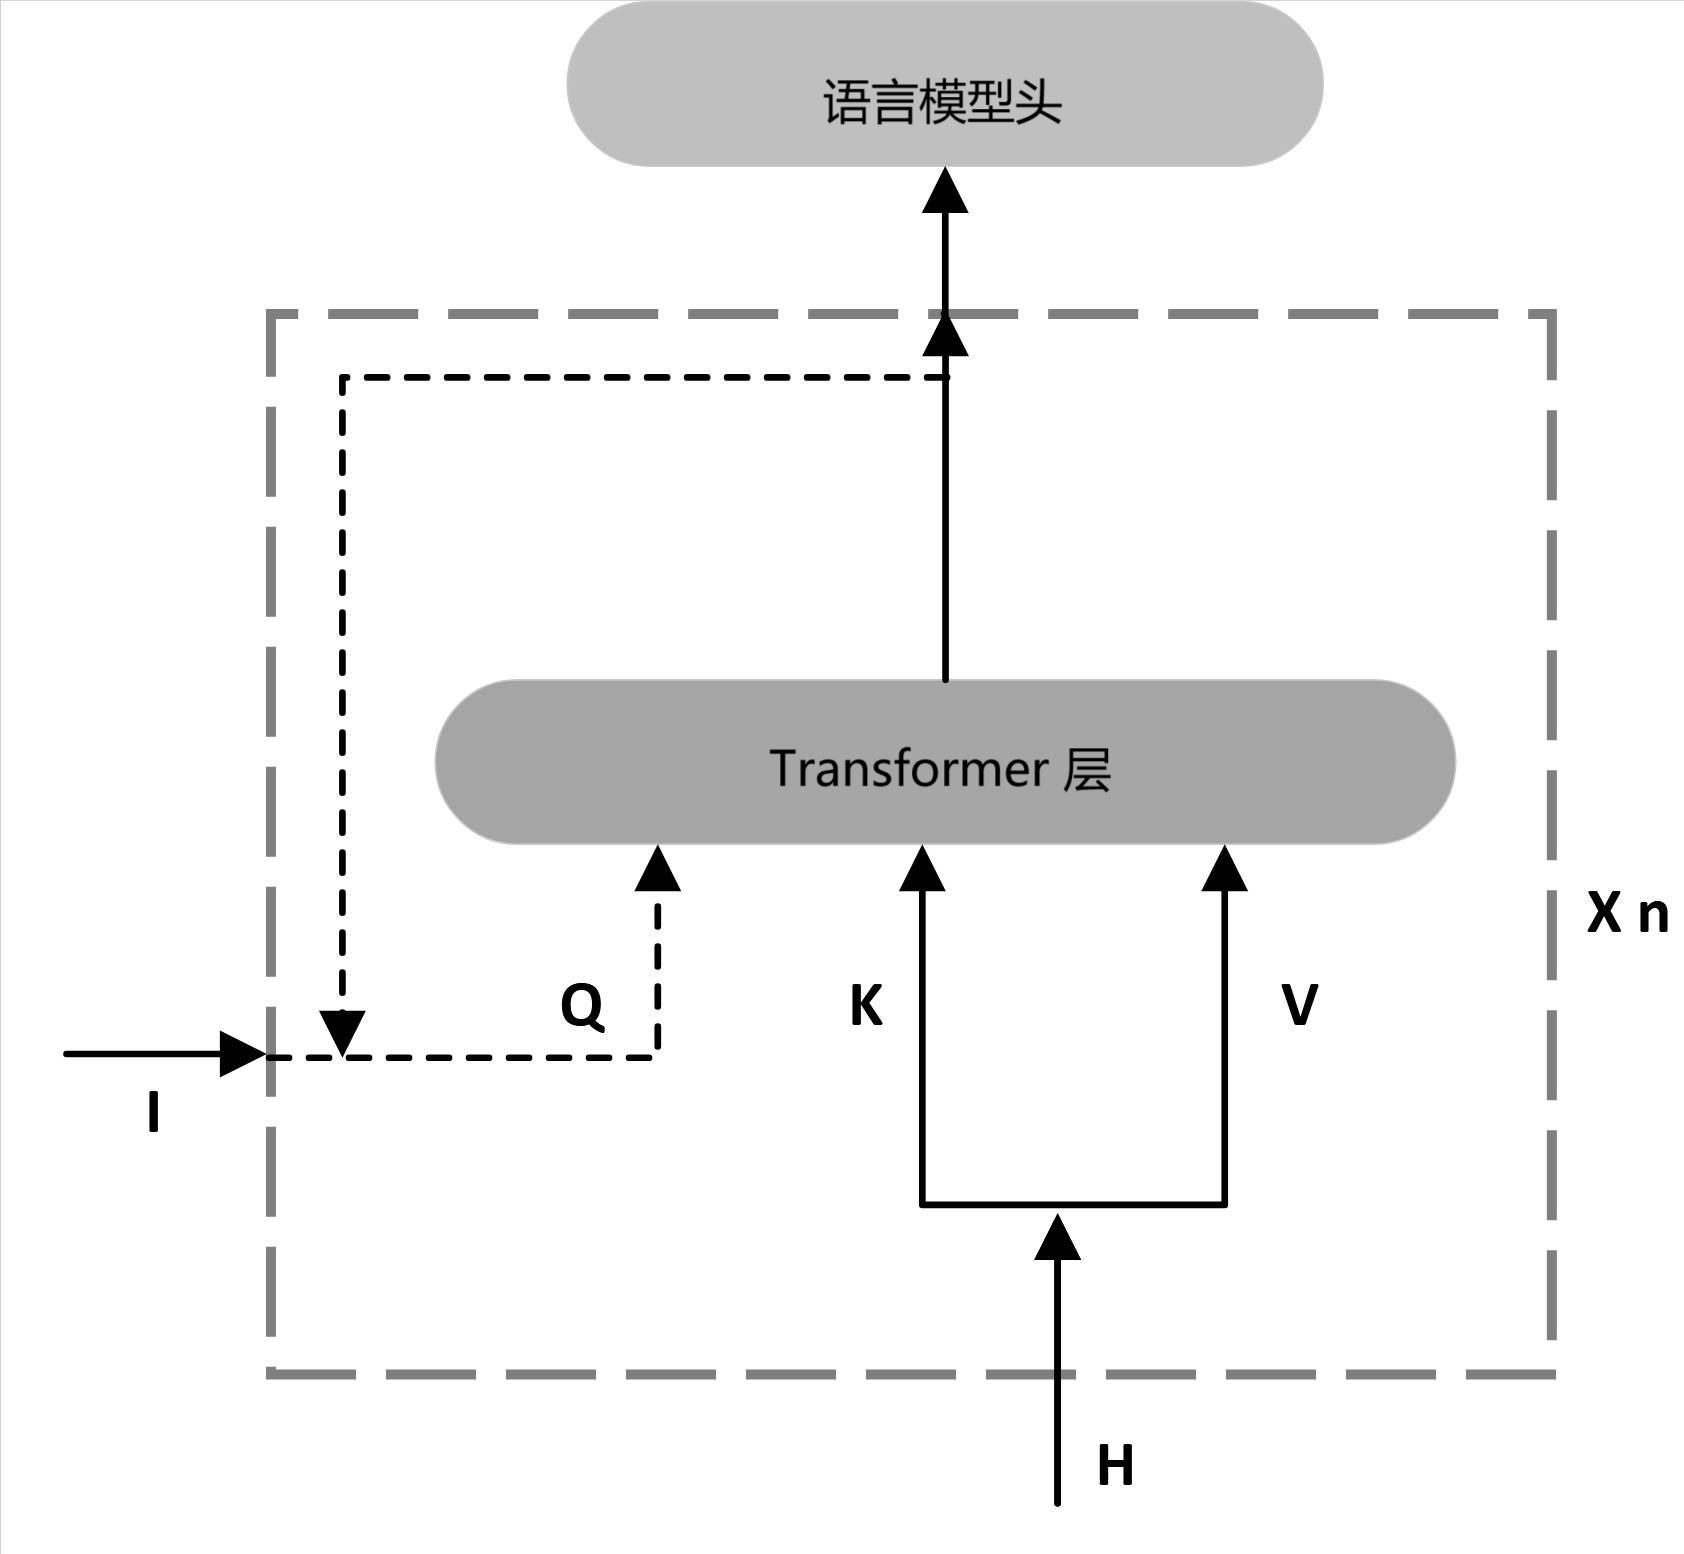
\includegraphics[trim={0.5mm 0.5mm 0.5mm 0.5mm},clip,width=0.58\linewidth]{figures/Model_EMD_S.jpg}
    % \label{fig:emd-b}
}

\caption{BERT 与 DeBERTa 解码层的比较 \cite{he_deberta_2021}}
\label{fig:emd}
\end{figure*}

将绝对位置信息整合到模型中可以通过两种主要方式实现。BERT 模型选择在输入层直接引入绝对位置信息。相较之下,DeBERTa 结构则在所有 Transformer 层之后、但在基于聚合的上下文词内容和位置嵌入解码掩码词的 Softmax 层之前,添加绝对位置信息,如图 \ref{fig:emd} 所示。这种创新架构使DeBERTa具备双重优势:一方面在全部Transformer层级中精准建模相对位置关系,另一方面在重构遮蔽标记时巧妙融合绝对位置特征作为辅助信号。正是基于这一独特机制,该模型将其核心解码模块命名为"增强型掩码解码器"(Enhanced Mask Decoder, EMD)。

\subsubsection{DeBERTa V3 模型}

由于 ELECTRA \cite{clark2020electrapretrainingtextencoders} 中的替换词元检测(Replaced Token Detection, RTD)和 DeBERTa 中的解耦注意力机制已被证实在预训练阶段具有较高的样本效率,DeBERTa V3 因而应运而生。该模型将原始 DeBERTa 中采用的掩码语言模型(Masked Language Modeling, MLM)目标替换为替换词元检测目标,以充分整合后者的优势。

基于 Transformer 的预训练语言模型通常在大规模文本数据集上进行训练,旨在通过自监督学习的目标来获取上下文中单词的表示,这一目标被称为掩码语言建模(Masked Language Modeling, MLM)\cite{devlin_bert_2019}。具体而言,考虑一个序列 \(X = \{x_i\}\),我们随机选择并掩盖其中 15\% 的词元,从而生成一个损坏后的序列 \(\tilde{X}\)。接下来,我们训练一个由参数 \(\theta\) 表示的语言模型,以基于 \(\tilde{X}\) 来预测被掩盖的词元 \(\tilde{x}\),以重建原始序列 \(X\):
\begin{align}
\max_{\theta} \log p_{\theta}(X|\tilde{X}) = \max_{\theta} \sum_{i \in \mathcal{C}} \log p_{\theta}(\tilde{x}_i = x_i|\tilde{X})
\end{align}
在此,\(\mathcal{C}\) 表示序列中被掩盖词元的索引集合。BERT 的研究者建议,对于被掩盖的词元,10\% 应保持不变,另有 10\% 则用随机选择的词元进行替换,其余的词元则用 \([MASK]\) 标记进行替换。

与 BERT 仅依赖单一的 Transformer 编码器并通过掩码语言模型进行训练的方式不同,ELECTRA 采用生成对抗网络(GAN)的框架,利用两个 Transformer 编码器进行联合训练。具体而言,其中一个编码器作为生成器,经过掩码语言模型的训练,而另一个编码器则作为判别器,通过词元级的二元分类器进行训练。生成模块负责合成干扰词元以填充输入序列中的掩码位置,经此扰动后的序列随即输入判别模块进行处理。在判别阶段,通过二元分类机制对每个词元进行溯源分析,判定其属于原始词元或生成模块合成的替代词元。生成模块和判别模块的参数分别定义为 \(\theta_G\)​ 与 \(\theta_D\)​,其中判别模块的优化目标被形式化为替换词元检测任务(Replacement Token Detection, RTD)。生成器的损失函数可以表示为:
\begin{align} 
L_{\text{MLM}} = \mathbb{E} \left( - \sum_{i \in \mathcal{C}} \log p_{\theta_G}(\tilde{x}_{i,G} = x_i|\tilde{\mathbf{X}}_G) \right)
\end{align}
\(\tilde{\mathbf{X}}_G\) 代表对原始输入序列 \(\mathbf{X}\) 实施 15\% 随机掩码处理后的生成器专用输入数据。

具体而言,判别器的输入序列构建过程如下:首先依据生成器输出的概率分布进行采样,随后用采样结果替换原序列中被掩码的词元位置。
\begin{align} 
\tilde{x}_{i,D} = \begin{cases} \tilde{x}_{i} \sim p_{\theta_G}(\tilde{x}_{i,G} = x_i|\tilde{\mathbf{X}}_G), & i \in \mathcal{C} \\ x_i, & i \notin \mathcal{C} \end{cases}
\end{align}

判别器的损失函数可表示为:
\begin{align}
L_{\text{RTD}} = \mathbb{E} \left( - \sum_{i} \log p_{\theta_D} \left( \mathbb{1}(\tilde{x}_{i,D} = x_i)|\tilde{X}_D, i \right) \right) 
\end{align}
在此,\(\mathbb{1}(\cdot)\) 表示指示函数,而 \(\tilde{X}_D\) 则是依据公式 3 构建的判别器输入。在 ELECTRA 模型中,损失函数 \(L_{\text{MLM}}\) 和 \(L_{\text{RTD}}\) 进行联合优化,整体损失 \(L\) 定义为 \(L = L_{\text{MLM}} + \lambda L_{\text{RTD}}\),其中 \(\lambda\) 是判别器损失 \(L_{\text{RTD}}\) 的权重参数,通常在 ELECTRA 中设定为 50。

此外,DeBERTa V3 采用了一种创新的梯度解耦嵌入共享(Gradient-Disentangled Embedding Sharing, GDES)方法,以替代最初在 ELECTRA 中提出的用于替换词元检测的词嵌入共享(Embedding Sharing, ES)策略。这一改进显著增强了 DeBERTa V3 的性能表现。

\begin{figure*}[htbp]
\centering  
\subfloat[嵌入共享]{
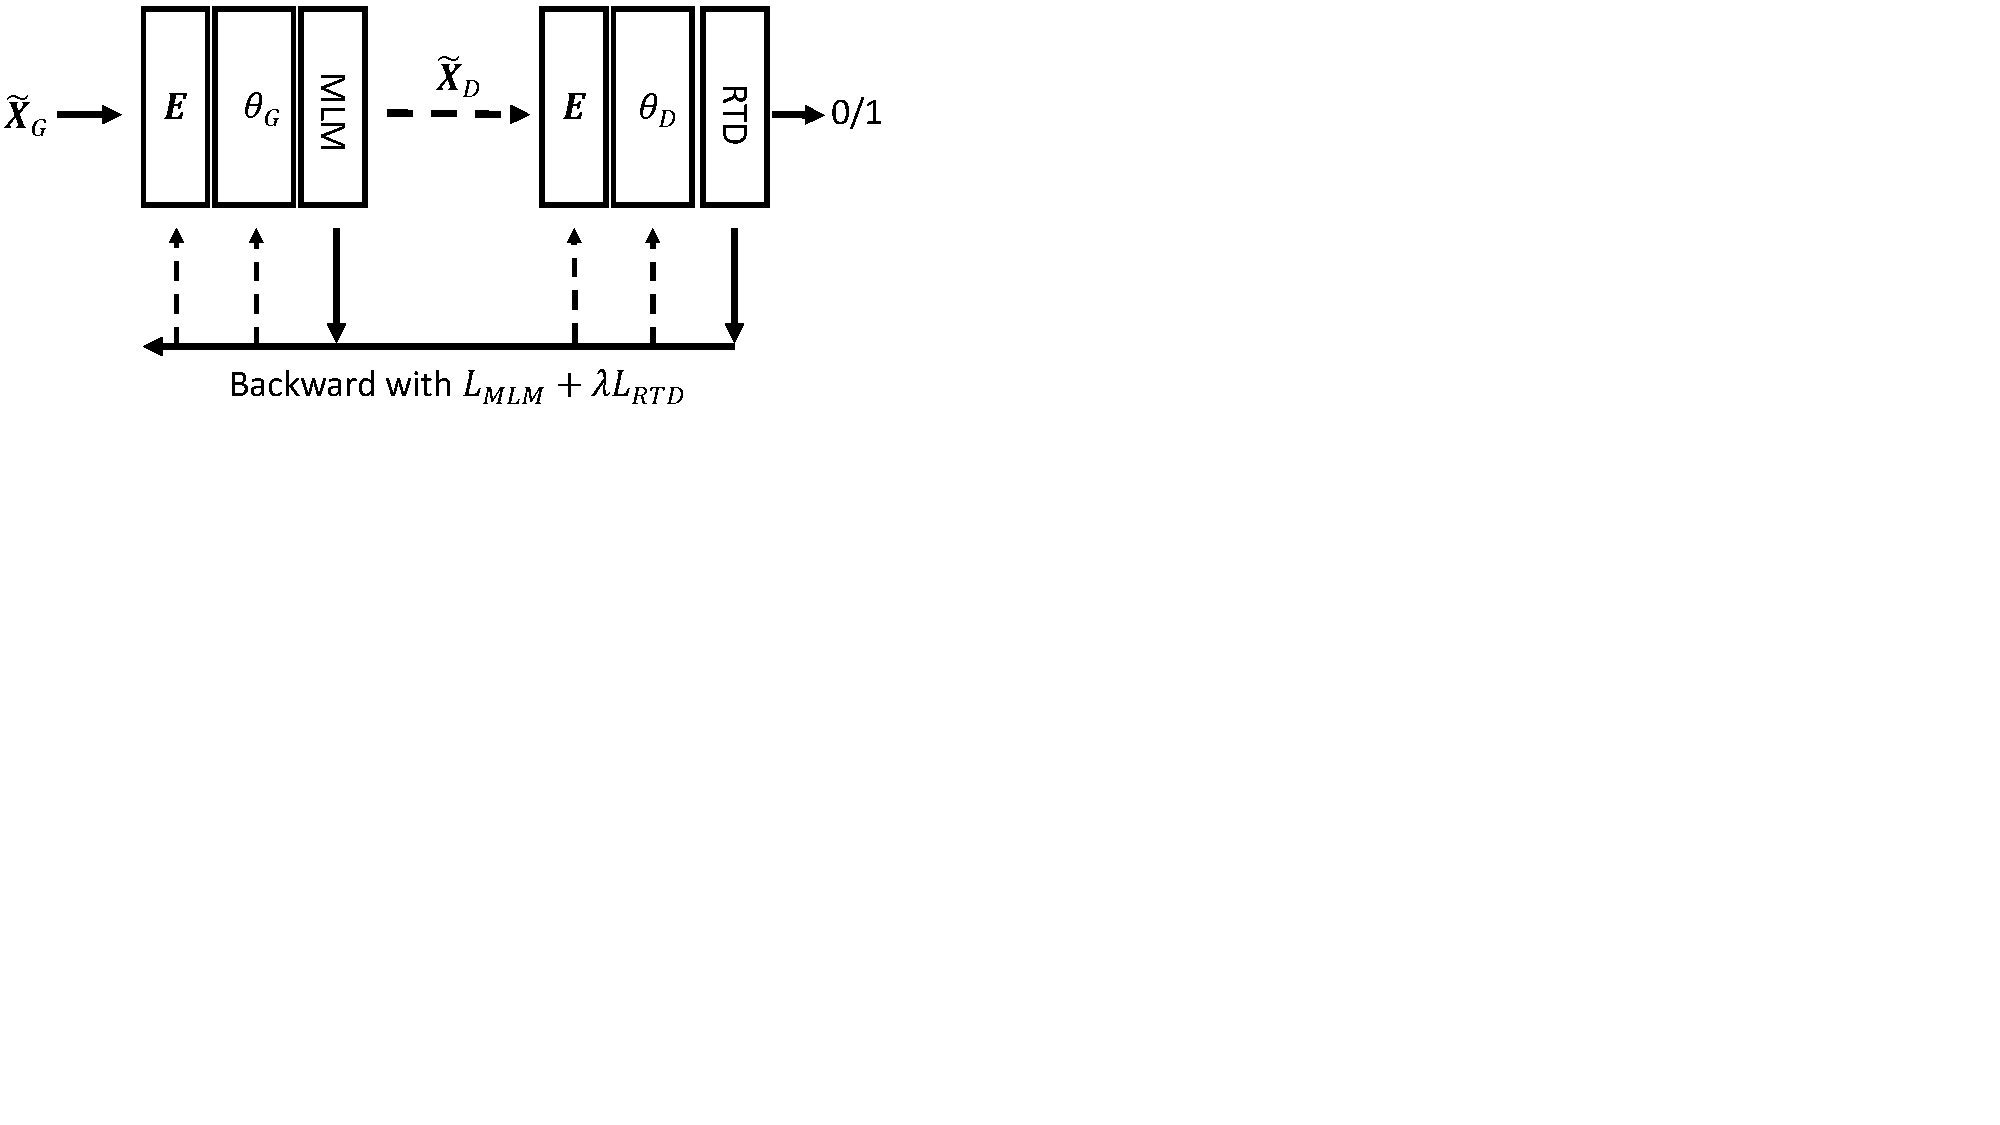
\includegraphics[width=0.31\linewidth,trim={0.1cm 11.8cm 18.5cm 0.1cm},clip]{figures/LRTD-a.pdf}
}
\hfill
\subfloat[无嵌入共享]{
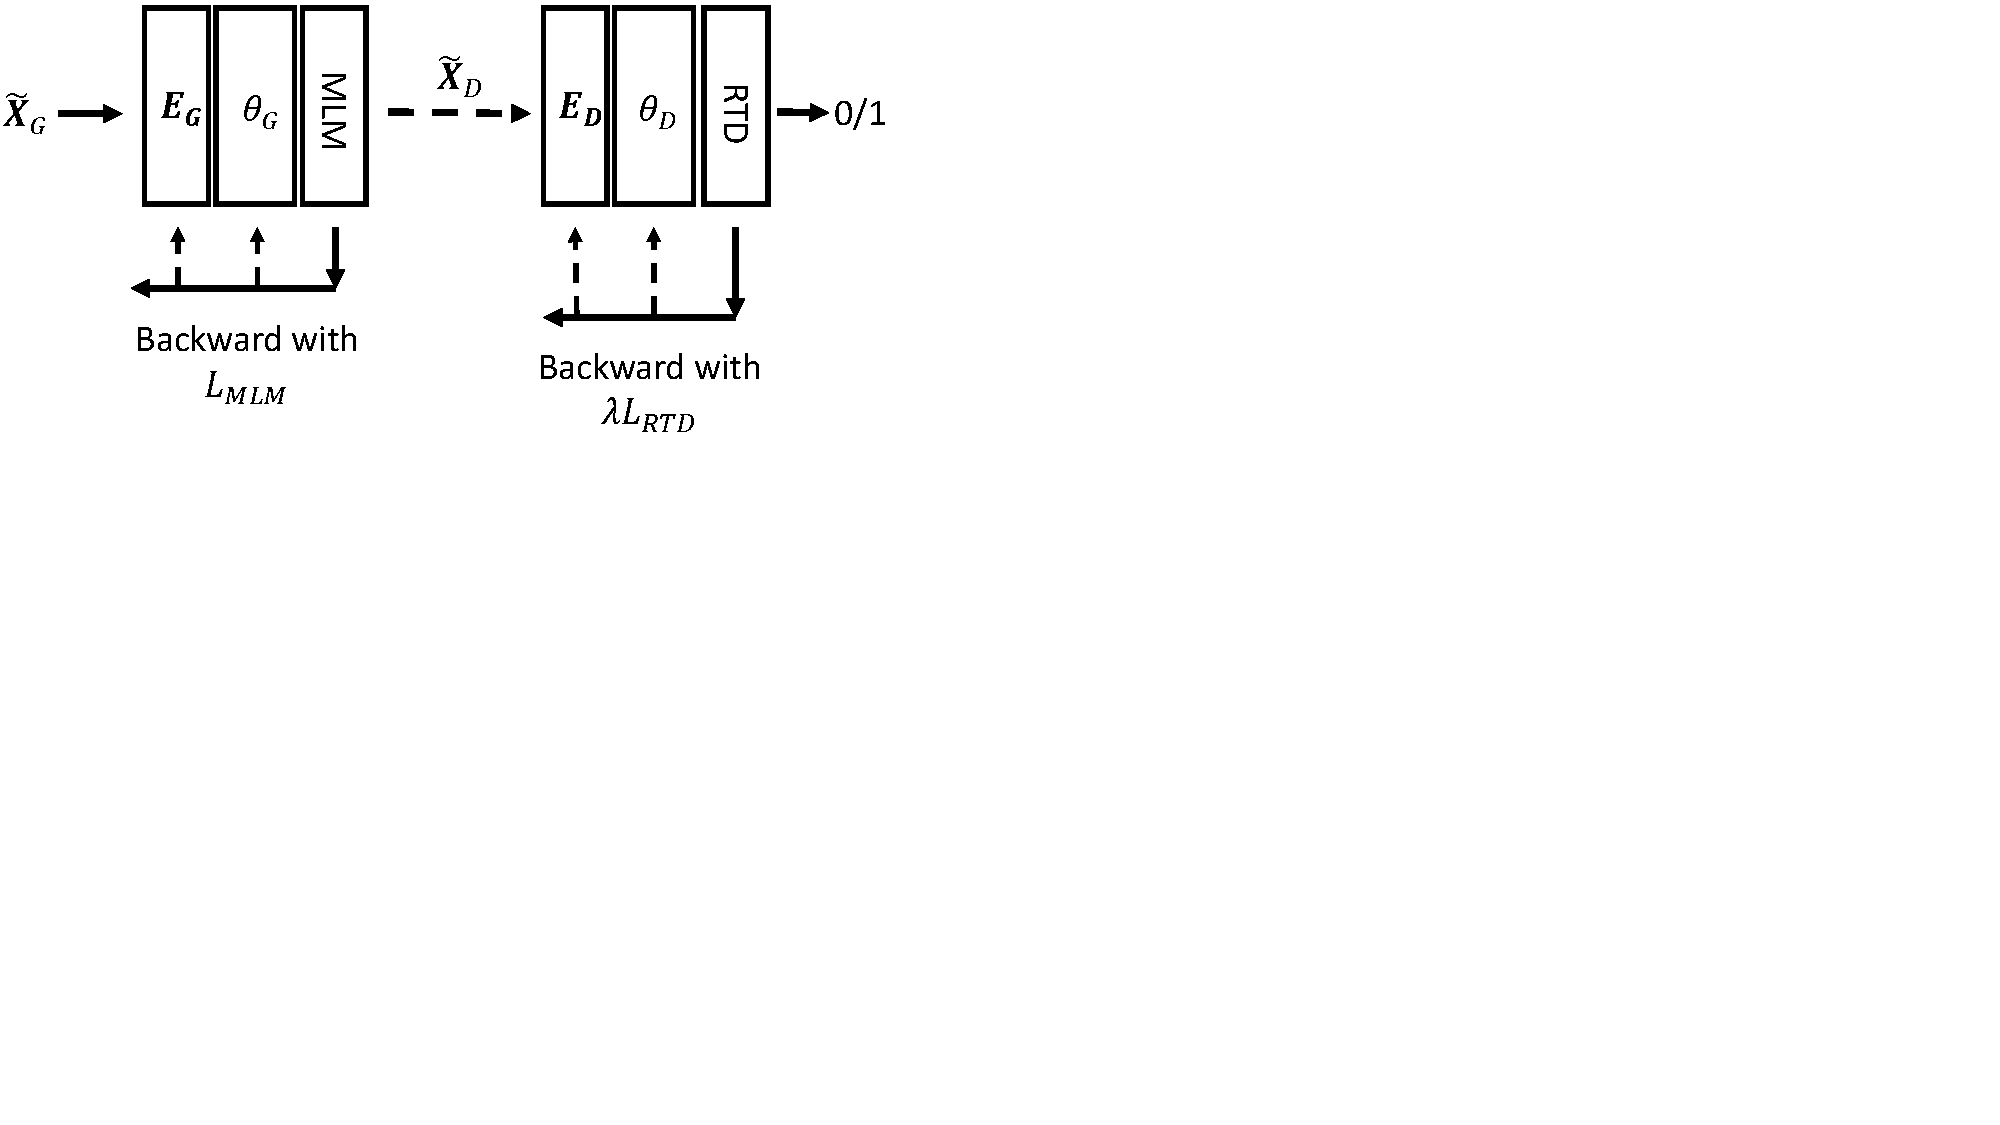
\includegraphics[width=0.31\linewidth,trim={0.1cm 11.7cm 18.5cm 0.1cm},clip]{figures/LRTD-b.pdf}
}
\hfill
\subfloat[梯度解耦嵌入共享]{
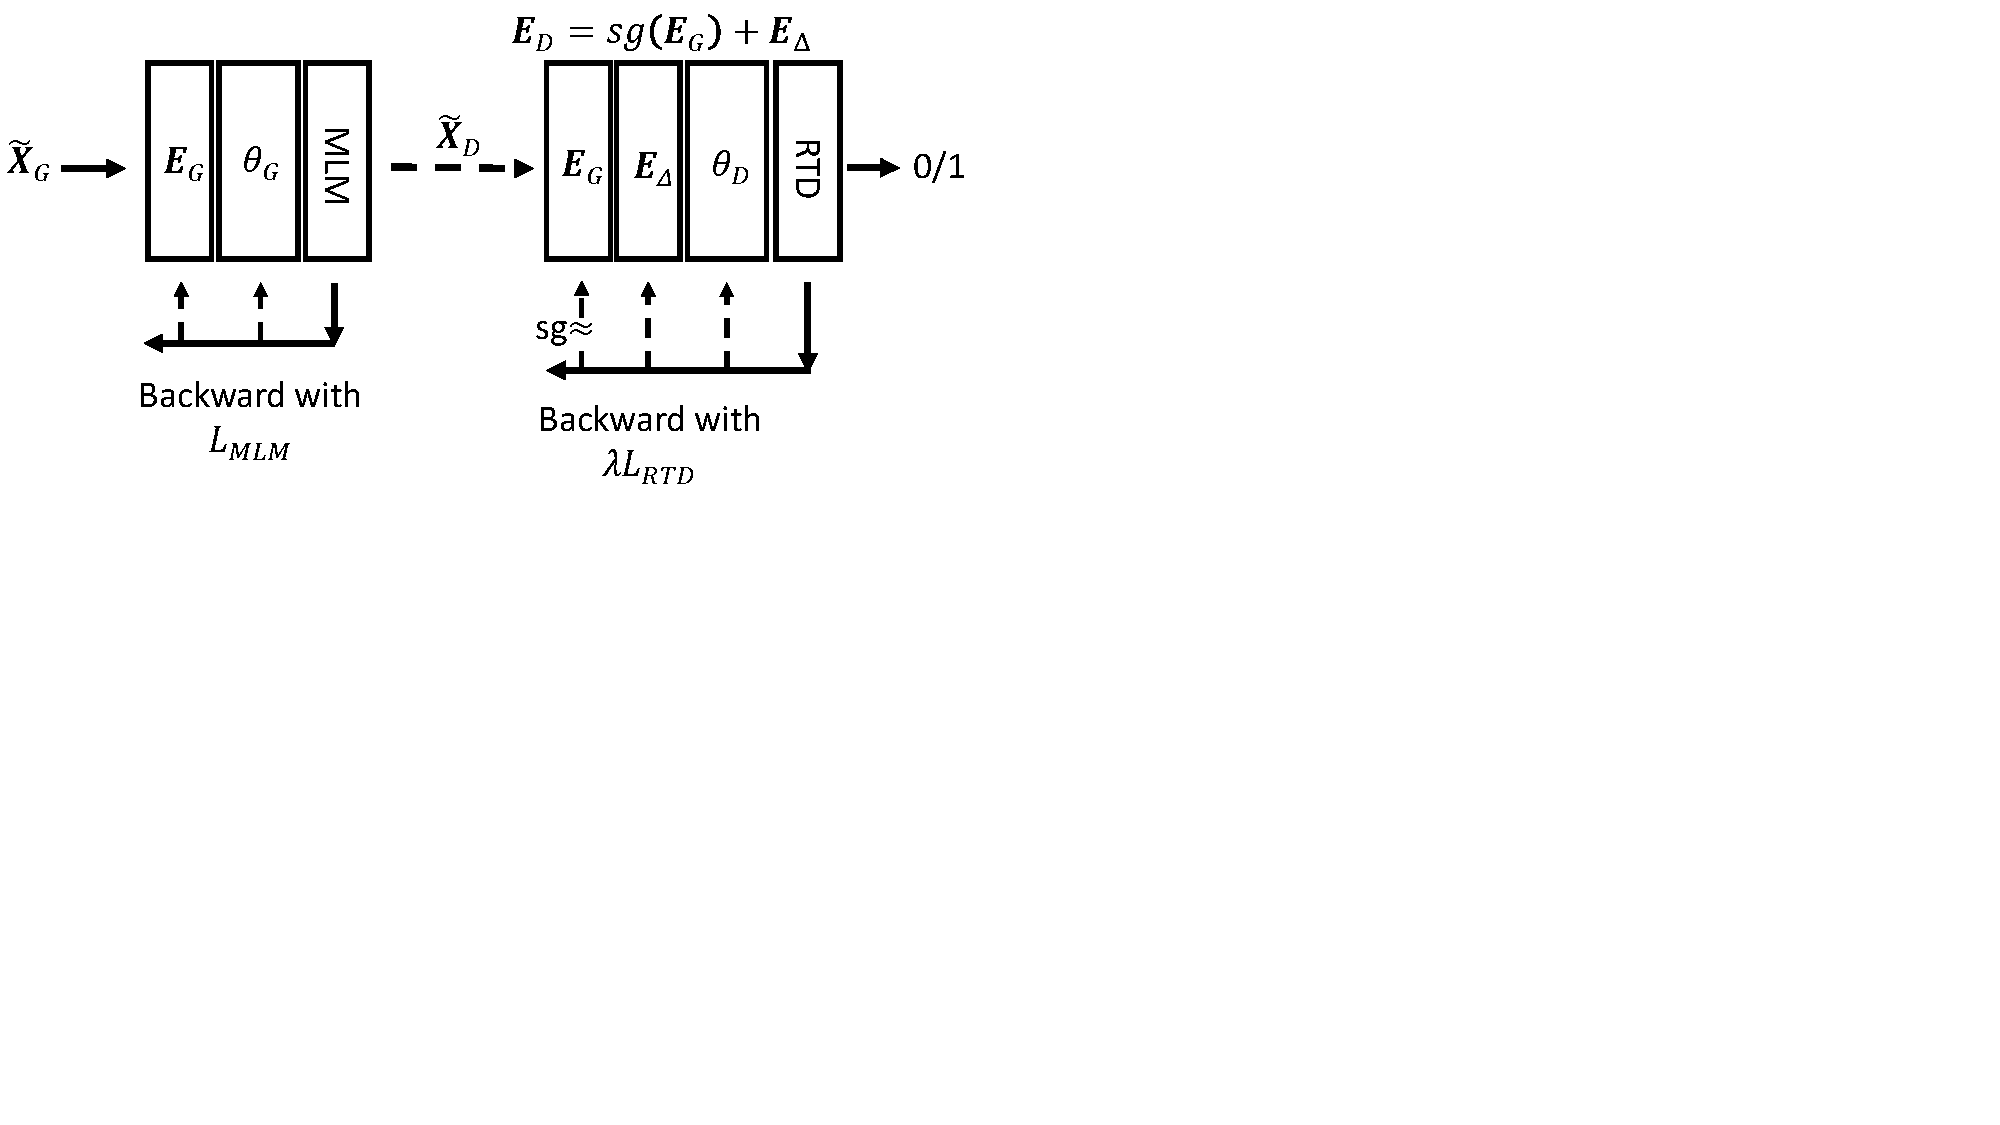
\includegraphics[width=0.31\linewidth,trim={0.1cm 10.4cm 17.5cm 0.1cm},clip]{figures/LRTD-c.pdf}
}
\caption{不同嵌入共享方法示意图 \cite{he2023debertav3improvingdebertausing}}
\label{fig:es}
\end{figure*}

DeBERTa V3 引入了一种名为梯度解耦嵌入共享(Gradient-Disentangled Embedding Sharing, GDES)的方法,旨在克服传统嵌入共享(Embedding Sharing, ES)和无嵌入共享(No Embedding Sharing, NES)所存在的不足,同时保留其优点。图 \ref{fig:es} 展示了不同嵌入共享策略的示意图。在嵌入共享(ES)策略中,参数 \(\mathbf{E}\)、\(\theta_G\) 和 \(\theta_D\) 在一次反向传播中依据损失函数 \(L_{\text{MLM}} + \lambda L_{\text{RTD}}\) 共同更新。而在无嵌入共享(NES)策略中,参数 \(\mathbf{E}_G\) 和 \(\theta_G\) 首先基于 \(L_{\text{MLM}}\) 进行反向传播更新,然后 \(\mathbf{E}_D\) 和 \(\theta_D\) 则依据 \(\lambda L_{\text{RTD}}\) 进行独立更新。与此不同,梯度解耦嵌入共享(GDES)方法首先根据 \(L_{\text{MLM}}\) 更新 \(\mathbf{E}_G\) 和 \(\theta_G\),接着则通过 \(\lambda L_{\text{RTD}}\) 和 \(\mathbf{E}_G\) 更新 \(\mathbf{E}_{\Delta}\) 和 \(\theta_D\)。在此过程中,停止梯度操作符 \(sg\) 被应用,以防止判别器对 \(\mathbf{E}_G\) 的更新。

如图 \ref{fig:es}(c)所示,梯度解耦嵌入共享方法允许生成器与判别器之间共享词嵌入,这使得两者能够从同一词汇表中学习并利用嵌入中蕴含的丰富语义信息。然而,与传统的嵌入共享方法相比,梯度解耦嵌入共享方法确保替换词元检测损失不会对生成器的梯度产生影响,从而避免了目标冲突带来的干扰和效率低下的问题。相反,该方法仅利用掩码语言模型损失来更新生成器的嵌入,确保生成器输出的一致性与连贯性。最终,梯度解耦嵌入共享方法能够实现与无嵌入共享相当的收敛速度,同时不牺牲嵌入的质量。

为实现梯度解耦嵌入共享,DeBERTa V3 将判别器的嵌入重新参数化为 \(\mathbf{E}_D = sg(\mathbf{E}_G) + \mathbf{E}_{\Delta}\),其中停止梯度算子 \(sg\) 防止梯度流经生成器的嵌入 \(\mathbf{E}_G\),仅更新残差嵌入 \(\mathbf{E}_{\Delta}\)。在训练过程中,\(\mathbf{E}_{\Delta}\) 被初始化为零矩阵,并依据无嵌入共享的训练流程进行模型训练。在每次迭代中,生成器首先为判别器生成输入,并利用掩码语言模型损失更新 \(\mathbf{E}_G\) 和 \(\mathbf{E}_D\)。随后,判别器在生成的输入上进行操作,并通过梯度解耦嵌入共享损失仅更新 \(\mathbf{E}_D\) 的参数 \(\mathbf{E}_{\Delta}\)。训练完成后,\(\mathbf{E}_{\Delta}\) 将被加到 \(\mathbf{E}_G\) 上,得到的矩阵作为判别器的最终嵌入 \(\mathbf{E}_D\)。

DeBERTa V3 进行了广泛的实验,以评估梯度解耦嵌入共享方法相较于嵌入共享和无嵌入共享的有效性。实验结果表明,梯度解耦嵌入共享是一种有效的权重共享策略,适用于结合掩码语言模型和替换词元检测的预训练语言模型。因此,DeBERTa V3 模型在 Kaggle 排行榜和深度学习领域展现出卓越的性能。在本实验中,使用的 DeBERTa 系列模型包括 DeBERTa-V3-Base 和 DeBERTa-V3-Large,其模型参数如表 \ref{tab:deberta-parameter} 所示。

\begin{table*}[htbp]
\centering
\caption{DeBERTa-V3-Base 和 DeBERTa-V3-Large 模型参数} \label{tab:deberta-parameter}
\begin{tabular}{lcc}
\toprule
               & \multicolumn{1}{l}{\textbf{DeBERTa-V3-Base} \cite{he2023debertav3improvingdebertausing}} & \multicolumn{1}{l}{\textbf{DeBERTa-V3-Large} \cite{he2023debertav3improvingdebertausing}} \\ \midrule
Transformer 层数 & 12                                           & 24                                            \\
隐藏层维度          & 768                                          & 1024                                          \\
词汇表大小          & 128K                                         & 128K                                          \\
主干网络参数量        & 86M                                          & 304M                                          \\
嵌入层参数量         & 98M                                          & 131M                                \\ \bottomrule         
\end{tabular}
\end{table*}

\section{大语言模型技术}
\label{sec:rw-llm}

\subsection{ChatGPT}
\label{sec:TOSWT-gen-chatgpt}

最早推出的 ChatGPT \cite{chatgpt},也被称为 GPT-3.5(Generative Pre-trained Transformer 3.5),是 OpenAI 在 GPT-3 的基础上进行优化而构建的大型语言模型(LLM)。该模型属于生成式预训练模型家族,基于 Transformer 架构,展现出在自然语言生成(NLG)、理解(NLU)以及多任务处理等方面的卓越性能,广泛应用于学术写作、代码生成和智能客服等多个领域。

ChatGPT 基于 Transformer 架构的神经网络设计,其核心特征在于自注意力机制(Self-Attention)的应用。这一机制能够有效捕捉文本序列中的长距离依赖关系,并支持并行计算,从而提高训练效率。研究表明,该模型的某些版本参数规模可达 1750 亿,通过构建深层网络结构并结合海量训练数据(包括互联网公开文本和学术文献等),显著提升了模型的性能表现。在训练方法上,ChatGPT 采用了“预训练与微调”的混合范式:首先通过无监督学习从大规模语料库中提取通用语言表征,随后结合有监督微调技术进行任务适配。此外,该模型创新性地引入了人类反馈强化学习 \cite{kaufmann2024surveyreinforcementlearninghuman}(Reinforcement Learning from Human Feedback, RLHF)方法,从而有效优化模型输出与人类价值观之间的对齐性。

ChatGPT(GPT-3.5)作为 OpenAI 首个面向公众的大规模对话式人工智能,具有里程碑式的技术发展意义。其历史贡献主要体现在三个方面:首先,它通过免费交互的形式使得具有 1750 亿参数的大型模型能力得以普及,用户在短短两个月内突破一亿,成为历史上增长最快的消费级应用;其次,借助于指令微调和人类反馈强化学习(RLHF)的技术创新,显著增强了模型对人类意图的对齐能力,为后续对话模型的训练框架奠定了基础;最后,其在代码生成、教育辅助等领域的跨领域应用展示了通用人工智能的潜力,例如成功通过美国律师考试并催生了 AIGC 产业生态。然而,随着后续模型(如 GPT-4 和 GPT-4o)的推出,其局限性逐渐显现:上下文窗口仅为 3000 词(而 GPT-4 可达 2.5 万词),在复杂推理和数学计算方面的准确率低于 GPT-4(例如在 LSAT 考试中,GPT-4 的得分高出 15\%);此外,其仅支持文本交互,缺乏多模态能力;知识的时效性受限于 2021 年的训练数据,且幻觉控制能力较弱,事实错误率比 GPT-4 高出约 40\%。这些不足促使模型向更大参数规模、更优对齐性及更低推理成本的方向不断演进。

从技术迭代的角度来看,GPT-3.5 的突破性在于首次验证了大规模预训练模型与人类反馈相结合的优化方案的可行性。然而,其单模态架构及有限的推理能力在专业领域的应用中逐渐显得不足。例如,OpenAI 推出的新一代模型 GPT-4 通过引入多模态处理和万亿级参数,在医学诊断、法律分析等任务中展现出更高的可靠性。而 GPT-4o 则进一步整合了音频和视频交互能力,实现了更为自然的人机交互体验。

\subsection{GPT4o}
\label{sec:TOSWT-gen-gpt4o}

GPT-4o \cite{gpt4o} 是 OpenAI 于 2024 年 5 月推出的下一代多模态大语言模型,其中的 "o" 代表 "omni"(全能),标志着其在文本、音频和视觉模态的端到端处理能力上取得了显著突破。该模型采用统一的 Transformer 架构,能够通过单一神经网络直接处理多模态输入(包括文本、图像和音频的任意组合),并生成文本、音频和图像输出的任意组合,从而消除了传统多模态系统中不同模型间转换所带来的延迟问题。GPT-4o 实现了跨文本、视觉和音频的端到端训练,意味着所有输入和输出均由同一神经网络处理。在技术层面,该模型通过改进的词元化(tokenization)方法,将音频特征和视频帧序列编码为与文本相同的表示形式,并利用多头注意力机制实现跨模态的语义关联,能够在低至 232 毫秒的时间内响应音频输入,平均响应时间为 320 毫秒,这与人类在对话中的反应时间相当。

与前代模型相比,GPT-4o 展现出三方面显著优势:首先,其多模态能力实现了质的飞跃,能够执行如图像内容分析生成食谱以及通过呼吸声识别情绪状态等复杂任务;其次,其非英语语言处理能力显著提升,支持 50 种语言的实时翻译,尤其在非拉丁语系文字(如韩语和阿拉伯语)的识别准确率提高超过 20\%;最后,其运行效率得到了显著优化,API 成本较 GPT-4 Turbo 降低了 50\%,推理速度提升了两倍。

\subsection{Gemini}
\label{sec:TOSWT-gen-gemini}

Gemini \cite{geminiteam2024geminifamilyhighlycapable} 是 Google DeepMind 开发的一系列多模态大语言模型,标志着谷歌在通用人工智能领域的重要进展。该系列模型于 2023 年 12 月正式推出,其核心创新在于采用原生多模态架构,能够同时处理文本、图像、音频、视频及代码五种信息类型。与传统多模态模型不同,Gemini 从预训练阶段起便利用统一的神经网络处理多模态输入,通过改进的词元化(tokenization)方法将不同模态的数据编码为统一表示,并通过多头注意力机制实现跨模态的语义关联。这一设计使其在复杂推理任务中表现卓越,例如能够理解手写的物理题解答并指出错误推理步骤,或将视觉信息转化为编程代码。在技术层面,Gemini 采用 TPUv4/v5e 加速器进行训练,其训练数据涵盖网络文档、学术文献和多语言语料,并通过人类反馈强化学习 \cite{kaufmann2024surveyreinforcementlearninghuman} (RLHF)优化输出的一致性。

尽管 Gemini 在多模态理解和复杂推理方面展现出优势,但仍存在一定的局限性。早期版本受到质疑,认为其测试分数夸大且演示视频存在剪辑问题,此外在非英语任务中的性能相对较弱。与后续模型相比,Gemini 缺乏动态更新机制,其在专业领域(如医学和法律)的微调效果有待提升。这些不足促使谷歌朝着更大参数规模、更低推理成本和更专业化的方向迭代,例如发布了开源模型 Gemma(20 亿/70 亿参数)。总体而言,Gemini 系列通过原生多模态架构和规模化训练基础设施,为通用人工智能的发展提供了重要的技术范式。

\subsection{Qwen}
\label{sec:TOSWT-gen-qwen}

通义千问 \cite{qwen2025qwen25technicalreport}(Qwen)是阿里云自主研发的一系列超大规模语言模型,作为中国人工智能领域的重要代表,其技术进步和产业应用充分体现了国产大模型的发展历程。该模型系列于 2023 年 4 月 11 日正式发布,其名称蕴含双重含义:“通义”象征着模型在跨领域知识理解方面的广泛适用性,而“千问”则源自中国古代百科全书《千问》,彰显其处理复杂问题的能力。在技术架构方面,通义千问采用了改进的 Transformer 结构,通过旋转位置编码 \cite{su2023roformerenhancedtransformerrotary}(RoPE)增强了对长序列的建模能力。此外,该模型创新性地结合了非绑定式嵌入(un-tied embeddings)与 RMSNorm 层进行优化,使其在 72B 参数版本中实现了 2048 个词元的上下文窗口支持。值得一提的是,其开源模型 Qwen1.5-110B 采用了稀疏专家混合(MoE)架构,并在 2024 年 5 月发布的 2.5 版本中,逻辑推理和代码能力较前一代提升了 16\% 和 10\%。

该模型的核心竞争力体现在三个主要方面:多模态融合、产业适配性以及开源生态系统的构建。在模态支持方面,通义千问2.0 已实现对文本、图像和音频的端到端处理,其多模态理解能力使其能够执行从商品设计草图生成营销文案等复杂任务。在产业应用方面,阿里云通过实施“云智一体”战略,将模型能力深度嵌入电商、医疗和金融等多个场景。例如,通义灵码智能编程助手能够完成 85\% 的常规代码生成任务,从而显著提升开发效率。在开源策略方面,截至 2025 年,通义千问已发布从 1.8B 到 110B 参数的七款开源模型,累计下载量超过 700 万次。其中,Qwen-72B 在 MMLU 基准测试中达到了与 Llama3-70B 相当的精度。

与同期国际模型相比,通义千问展现出显著的差异化特征。其训练数据中包含超过 30\% 的高质量中文语料,使其在古文解析和中文创意写作等任务上表现优于同等规模的 GPT-3.5 模型。在商业应用方面,通过实施 API 价格策略(2 元/1M tokens)及轻量化部署方案(例如与联发科天玑9300芯片的适配),显著降低了企业的使用门槛。然而,该模型在处理非拉丁语系的多语言任务时,其准确率仍比 GPT-4 低约 15\%。这些技术优势使通义千问成为中国大模型技术自主创新与全球竞争的重要案例,其发展路径为学术界在 AI 技术产业化方面的研究提供了典型的参考样本。

\subsection{DeepSeek}
\label{sec:TOSWT-gen-ds}

DeepSeek V3 \cite{deepseekai2024deepseekv3technicalreport} 是中国深度求索公司(DeepSeek)于2024年12月发布的新一代多模态大语言模型,标志着国产大模型在技术创新与成本控制方面的重要里程碑。该模型采用混合专家(MoE)架构,总参数量达到6710亿,其中每个词元激活370亿参数,通过动态路由机制实现计算资源的高效分配。在技术层面,DeepSeek V3 创新性地结合了多头潜在注意力机制(MLA)与 FP8 混合精度训练。前者通过低秩压缩键值对有效降低内存占用,后者则在矩阵乘法等计算密集型操作中采用 FP8 格式,使得训练成本控制在557.6万美元,仅为 GPT-4o 等主流模型的十分之一。在14.8万亿 token 的预训练基础上,模型通过监督微调和强化学习进一步优化性能,其生成速度达到60 TPS(每秒事务处理量),较前代 V2.5 提升了三倍,显著改善了交互的流畅性。

在性能表现方面,DeepSeek V3 展现出在多个领域的竞争优势。在知识类任务(如 MMLU 和 GPQA)中,其表现接近于 Claude-3.5-Sonnet,而在数学竞赛(如 AIME 2024 和 CNMO 2024)中,其成绩超越了所有开源和闭源模型。此外,其代码生成能力可与 85\% 的人类编程选手相媲美。特别是在中文处理方面,凭借 30\% 的高质量中文语料进行训练,该模型在古文解析和创意写作等任务中优于同等规模的国际模型。2025年3月发布的 V3-0324 版本进一步增强了前端开发能力,能够根据单一提示自动生成包含交互控件和赛博朋克风格界面的完整网站,开发者将其誉为“编码领域的标杆”。该模型支持 128K 的上下文窗口(开源版),在长文本理解任务(如 DROP 和 LongBench v2)中的平均表现领先于行业标准。

DeepSeek V3 的商业化与开源策略是其另一显著特色。其 API 定价极具竞争力,输入和输出词元的成本分别为每百万词元 0.27 美元和 1.10 美元,较国际同类产品降低超过 50\%。该模型采用 MIT 开源协议,允许商业用途及二次开发,截至 2025 年,已实现 700 万次下载,促进了 AI 技术在边缘设备上的部署。其应用场景涵盖智能编程(如通义灵码助手)、金融风险控制及教育辅导等多个领域。在电商平台的数据分析场景中,该模型能够实时识别欺诈交易并生成可视化报告。

尽管 DeepSeek V3 的表现十分出色,但其仍存在一定局限性,尤其是在处理复杂音频和视觉输入时,其幻觉率比文本模态高出约 20\%。然而,DeepSeek V3 现有的诸多优势特性使其成为研究 AI 技术普惠化与计算效率优化的典型案例,为中国大模型在全球竞争中的发展提供了重要参考。

\section{AI 生成文本检测技术}
\label{sec:llmdetect}

大型语言模型(LLMs)的迅速发展促使对检测 AI 生成文本的方法进行深入研究。在 ChatGPT 发布之前,GLTR \cite{gehrmann_gltr_2019} 作为一种文本检测工具,通过一系列统计分析技术识别由不同采样策略生成的文本特征。GLTR 有效地将人类对生成文本的检测准确率从 54\% 提升至 72\%,彰显了其在帮助非专业人士区分人类与机器生成内容方面的实用性。

另一个重要的贡献是人类 ChatGPT 比较语料库 \cite{guo_how_2023}(HC3),该语料库是在 ChatGPT 发布后开发的。HC3 数据集包含来自人类专家与 ChatGPT 的数万个响应,涵盖金融、医学和法律等多个领域。这一数据集使得对 ChatGPT 的响应与人类输出进行全面评估成为可能,从而揭示了 LLMs 的能力与局限性。此外,HC3 还促进了检测系统的发展,旨在识别文本是由 ChatGPT 还是人类生成的。

LLM-Detector \cite{wang_llm-detector_2024} 针对现有人工智能生成文本检测模型所面临的挑战进行了研究,这些模型通常因领域内过拟合而在领域外表现不佳。该研究通过收集人类专家和多种大语言模型的回复,基于大型语言模型提出了一种新颖的检测方法,利用指令调优来增强文档级和句子级的检测能力。实验结果表明,该方法在性能上显著优于基线方案,展现出强大的泛化能力。

SeqXGPT \cite{wang_seqxgpt_2023} 通过构建一个包含大语言模型生成句子与人类写作内容的数据集,引入了句子级检测挑战。该方法利用来自白盒 LLMs 的对数概率列表,结合卷积网络和自注意力机制以提高检测准确性。结果显示,SeqXGPT 在句子和文档级检测任务中均优于现有方法,进一步强调了有效检测机制的必要性。

针对人工智能生成文本来源追踪的问题 \cite{li_origin_2023},已有研究提出了一种创新的算法,旨在检测和追踪人工智能生成的内容。该方法通过对比特征有效区分由不同模型生成的文本,能够在白盒和黑盒环境中均发挥作用。研究结果突显了人工智能部署所带来的伦理影响,以及追踪生成文本来源机制的重要性,为关于人工智能系统问责制的持续讨论提供了重要的理论支持。

然而,现有的方法 \cite{gehrmann_gltr_2019, guo_how_2023, wang_llm-detector_2024, wang_seqxgpt_2023} 尚未满足我们对文本来源于特定大型语言模型的检测需求。大多数研究在分类任务上表现较为粗糙,仅能识别文本是由人类还是机器生成,无法进一步确定文本的具体来源。尽管少部分研究 \cite{li_origin_2023} 实现了识别文本来源于特定大型语言模型的目标,但其实现方式依赖于白盒测试,必须获取与待检测模型一致或相似的模型生成的特征向量才能进行判断。在当前大多数大型语言模型均为闭源的环境下,这种方法几乎缺乏扩展性和可操作性。

\section{本章小结}
\label{sec:rw-conclusion}

本章回顾了当前自然语言处理领域的相关工作,重点聚焦于文本生成技术和预训练语言模型的进展。首先,我们深入分析了Transformer架构的优势,强调了其在大语言模型中的广泛应用。自2017年提出以来,Transformer因其卓越的并行处理能力和长距离依赖建模能力,迅速成为自然语言处理研究的核心。通过自注意力机制,Transformer能够有效捕捉输入序列中各个部分之间的关系,从而显著提高了模型在处理大规模文本数据时的训练效率和表达能力。

随后,我们详细讨论了BERT模型的结构及其在预训练和微调过程中的创新。BERT不仅在机器阅读理解等多个任务中取得了显著的性能提升,还引入了预训练-微调的二阶段训练范式,使得模型能够在预训练阶段学习通用的语言表示,而在特定任务中进行微调。这一策略极大地提升了模型的适应性和性能,标志着自然语言处理领域的一次重大变革。在预训练语言模型的讨论中,我们提及了如GPT、RoBERTa和DeBERTa等模型的相继出现,这些模型在BERT的基础上进行了不同程度的改进,进一步推动了预训练模型的研究和应用。

此外,我们介绍了多种大型语言模型,包括 ChatGPT、GPT4o、Gemini、Qwen 和 DeepSeek。研究表明,大语言模型正沿着多模态融合、计算效率优化和专业化应用三个维度持续演进:从ChatGPT的单模态文本处理到GPT-4o的端到端多模态交互,体现了模态整合能力的突破;Gemini的原生多模态架构与DeepSeek V3的混合专家设计展示了计算效率的优化路径;而通义千问的产业适配策略则凸显了专业化应用的重要性。这些模型在提升语言理解、跨模态推理等核心能力的同时,仍面临幻觉控制、多语言处理等方面的技术挑战,其发展轨迹为后续研究提供了重要的技术参照和产业化启示。这五个大语言模型这些模型将在后面的章节中用于构建改写文本数据集。

最后,本章探讨了AI生成文本的检测技术,介绍了多种现有方法及其在实际应用中的效果与局限性。尽管GLTR、HC3、LLM-Detector、SeqXGPT等工具在识别生成文本方面取得了一定的成效,但仍面临特定大型语言模型检测的挑战。尤其是在当前许多大型语言模型为闭源的环境下,现有方法在文本来源追踪和特定模型检测方面的适用性显得尤为重要。

综上所述,本章的讨论为理解当前技术状态及未来研究方向提供了重要视角,为本论文的研究奠定了坚实的基础。通过对Transformer架构、BERT模型及AI文本检测技术的全面回顾,我们为后续的研究和实验提供了必要的理论支持和实践指导。